\chapter{Neodlučivost}\label{ch:ne}

%\section{Teoremi ekvivalencije}

Dokazali smo brojne teoreme koji pokazuju ekvivalentnost različitih modela iz\-ra\-čun\-ljiv\-os\-ti. Za početak ih sve objedinimo na jednom mjestu. Najvažniji je svakako onaj koji govori o brojevnim funkcijama, odnosno karakterizira skup $\mathcal Comp$.

\begin{teorem}[Teorem ekvivalencije za brojevne funkcije]
Neka je $k\in\N_+$, te\, $\f f\colon\N^k\rightharpoonup\N$ brojevna funkcija mjesnosti $k$. Tada su sljedeće tvrdnje ekvivalentne:
\begin{itemize}
    \item[\texttt{\textup{(r)}}] $\f f$ je RAM-izračunljiva (\,$f\in\mathcal Comp_k$);
    \item[\texttt{\textup{(m)}}] $\f f$ je makro-izračunljiva (postoji makro-algoritam koji računa $\f f$);
    \item[\texttt{\textup{(p)}}] $\f f$ je parcijalno rekurzivna (\,$\f f$ je dobivena iz inicijalnih pomoću konačno mnogo primjena kompozicije, primitivne rekurzije i minimizacije);
    \item[\texttt{\textup{(i)}}] $\f f$ ima indeks (postoji $e\in\N$ takav da je $\f f=\kf e^k$);
    \item[\texttt{\textup{(t)}}] $\beta\f f$ je Turing-izračunljiva (postoji Turingov stroj koji računa $\beta\f f$).
\end{itemize}
\end{teorem}
\begin{proof}
Sve bitno u ovom teoremu smo već dokazali. Ponovimo samo glavne ideje.

\begin{labeling}{\texttt{(a$\Rightarrow$b)}}
    \item[\texttt{(r$\Rightarrow$m)}] Ovo je trivijalno: $\mathcal Prog\subset\mathcal{MP}rog$ (svaki RAM-program je ujedno i makro-program) --- napomena~\ref{nap:rem}.
    \item[\texttt{(m$\Rightarrow$r)}] Svaki makro-program $Q\in\mathcal{MP}rog$ ekvivalentan je svojem spljoštenju $Q^\flat\in\mathcal Prog$ --- teorem~\ref{tm:rem}.
    \item[\texttt{(p$\Rightarrow$r)}] \emph{Postorder}-obilaskom njene simboličke definicije, kompajliramo funkciju $\f f$ u RAM-program --- teorem~\ref{tm:pir}.
    \item[\texttt{(r$\Rightarrow$i)}] Ako RAM-program $P\in\mathcal Prog$ računa $\f f$, tada je njegov kod $e:=\kprog P\in\f{Prog}$ jedan indeks za $ \f f$ --- propozicija~\ref{prop:computeind}.
    \item[\texttt{(i$\Rightarrow$p)}] Funkcija $\f f^k$ s indeksom $e$ dobivena je kompozicijom $\f{comp}_k$, konstante $\f C_e^k$ i koordinatnih projekcija --- korolar \ref{kor:iip}.
    \item[\texttt{(t$\Rightarrow$p)}] Funkciju $\f f$ možemo dobiti kompozicijom iz parcijalno rekurzivnih funkcija $\f{blh}$, $\N\beta\f f$ i $\f{bin}^k$ --- teorem~\ref{tm:btip}.
    \item[\texttt{(p$\Rightarrow$t)}] Funkciju $\N\beta\f f$ možemo dobiti restrikcijom na $\im{\f{bin}^k}$ kompozicije funkcija $\f{bin}^1$, $\f f$ i $\f{arg}_1$,~\ldots, $\f{arg}_k$ --- teorem~\ref{tm:pibt}.
\end{labeling}
Dijagramatski, usmjeren graf
\begin{tikzcd}
\t r
\arrow[leftrightarrow]{d}
\arrow{dr}
&
\t p
\arrow{l}
&
\t t
\arrow[leftrightarrow]{l}
\\
\t m
&
\t i
\arrow{u}
\end{tikzcd} je jako povezan.
\end{proof}

Za jednomjesne funkcije imamo korolar~\ref{kor:peuf}, koji je zgodniji zbog jednočlane abecede i bijektivnosti kodiranja. Za dokaz ekvivalencije parcijalne rekurzivnosti i Turing-izračunljivosti koristili smo ekvivalenciju brojevnog i jezičnog modela za jezične funkcije.

\begin{teorem}[Teorem ekvivalencije za jezične funkcije]
Neka je $\Sigma\not=\emptyset$ abeceda, te $\varphi\colon\Sigma^*\rightharpoonup\Sigma^*$ jezična funkcija nad njom. Tada su sljedeće tvrdnje ekvivalentne:
\begin{itemize}
    \item[\texttt{\textup{(T)}}] $\varphi$ je Turing-izračunljiva;
    \item[\texttt{\textup{(P)}}] $\N\varphi$ je parcijalno rekurzivna;
    \item[\texttt{\textup{(R)}}] $\N\varphi$ je RAM-izračunljiva.
\end{itemize}
\end{teorem}
\begin{proof}
Napomenimo, druga i treća stavka zapravo predstavljaju po $(\card\Sigma)!$ tvrdnji --- po jednu za svako kodiranje od $\Sigma$ --- ali sve su one ekvivalentne po korolaru~\ref{kor:ikojiNSigma}.

Opet, sve bitno je već dokazano; slijedi rekapitulacija glavnih ideja.
\begin{labeling}{\texttt{(A$\Rightarrow$B)}}
\item[\texttt{(T$\Rightarrow$P)}] Kodirajući sve dijelove Turing-izračunavanja s rječju zadanog koda, dobijemo parcijalnu rekurzivnost funkcije $\N\varphi$ --- teorem~\ref{tm:tikp}.
\item[\texttt{(P$\Rightarrow$R)}] Jednostavno kompajliramo funkciju $\N\varphi$ u RAM-program --- teorem~\ref{tm:pir}.
\item[\texttt{(R$\Rightarrow$T)}] Transpiliranjem RAM-programa koji računa $\N\varphi$, u pet faza dobijemo Turingov stroj koji računa $\varphi$ --- teorem~\ref{tm:krit}.\qedhere
\end{labeling}
\end{proof}

Karakteristična funkcija je totalna, dakle za izračunljive jezike mora biti rekurzivna.

\begin{teorem}[Teorem ekvivalencije za jezike]
Neka je $\Sigma\not=\emptyset$ abeceda, te $L\subseteq\Sigma^*$ jezik nad njom. Tada su sljedeće tvrdnje ekvivalentne:
\begin{itemize}
    \item[\texttt{\textup{(\textsc r)}}] relacija $\kr L:=\{\kr w\mid w\in L\}$ je rekurzivna;
    \item[\texttt{\textup{(\textsc o)}}] postoji Turingov odlučitelj $(Q,\Sigma,\Gamma,\bl,\delta,q_0,q_\mathit{true},q_\mathit{false})$ koji prepoznaje $L$.
\end{itemize}
\end{teorem}
\begin{proof}
Kao i u prethodnom teoremu, stavka \texttt{(\textsc r)} je zapravo $(\card\Sigma)!$ tvrdnji. One su ekvivalentne po tranzitivnosti, jer je svaka od njih ekvivalentna sa stavkom \texttt{(\textsc o)}.
\begin{labeling}{\texttt{(\textsc a$\Rightarrow$\textsc b)}}
\item[\texttt{(\textsc r$\Rightarrow$\textsc o)}] Malom modifikacijom kraja konstrukcije transpiliranog Turingovog stro\-ja koji računa $\N^{-1}\chi_{\kr L}$ dobijemo odlučitelj --- teorem~\ref{tm:krio}.
\item[\texttt{(\textsc o$\Rightarrow$\textsc r)}] Malom modifikacijom kodiranja stanja, funkcije prijelaza i Turing-iz\-ra\-ču\-na\-va\-nja odlučitelja dobijemo rekurzivnost od $\kr L$ --- teorem~\ref{tm:oikr}.\qedhere
\end{labeling}
\end{proof}

Još uvijek ostaje otvoreno pitanje što je s jezicima koje prepoznaju općeniti Turingovi strojevi, koji mogu i zapeti u beskonačnoj petlji (štoviše, kažemo da je ulazna riječ u jeziku Turingovog stroja ako i samo ako se to ne dogodi). Prema definiciji~\ref{def:Tcomputefi}, ti jezici su zapravo \emph{domene izračunljivih jezičnih funkcija}. Njihov status razriješit ćemo u točki~\ref{sec:relang}.

\begin{napomena}[{name=[kod problema zaustavljanja završno stanje trake nije bitno]}]\label{nap:re0}
Formalno, morali bismo još osigurati da im traka na kraju bude oblika $v\bl\ldots$ za $v\in\Sigma^*$, ali nije teško vidjeti, tehnikama koje se obrade u proučavanju formalnih jezika, da za svaki Turingov stroj (koji ne računa nužno neku funkciju) postoji Turingov stroj koji stane za točno iste ulaze, ali s praznom trakom ($v=\varepsilon$).

Skica dokaza: uvedemo novi znak \t/ u radnu abecedu i proglasimo ga prazninom (znak $\bl$ time postaje običan znak radne abecede), te za svaki prijelaz koji čita bivšu prazninu $\delta(p,\bl)=(q,\gamma,d)$ dodamo prijelaz $\delta(p,\t/)=(q,\gamma,d)$ (pisanja praznina ostavimo na $\bl$). Semantički, i $\bl$ i \t/ su sada praznine, ali stroj ne može napisati \t/ na traku --- odnosno, jedine pojave znaka \t/ na traci su tamo gdje stroj još nije bio. Kako su pomaci mogući samo na susjedne ćelije, nosač takve trake je nužno povezan.

Sada na bivše završno stanje dodamo fragment koji odlazi desno do prvog znaka \t/ (zna da su nadalje samo praznine), i vraća se lijevo, zamjenjujući sve znakove s \t/. Kada u tom stanju pročita \t/, stane jer je došao do lijevog ruba trake (taj \t/ sigurno nije mogao prije zapisati).
\end{napomena}

Već smo rekli da domene izračunljivih brojevnih funkcija ne moraju biti izračunljive --- recimo, $HALT=\dom{\f{univ}}$ nije izračunljiva, što ćemo ubrzo dokazati --- pa je za očekivati da to vrijedi i za općenite Turing-prepoznatljive jezike. Preciznije ćemo taj fenomen opisati kad uvedemo rekurzivno prebrojive relacije.

\section{\texorpdfstring{Church--\!Turingova teza}{Church-Turingova teza}}
Nakon toliko dokazanih implikacija oblika "ako je funkcija izračunljiva u nekom modelu, onda je izračunljiva i u drugom modelu", počinjemo uočavati određene obrasce u definicijama i dokazima.

%\subsection{Shematski prikaz izračunavanja}

Algoritam $\mathcal A$ je uglavnom opisan pomoću stroja (diskretnog dinamičkog sustava) s prebrojivim skupom mogućih konfiguracija $C$, tako da se svaka konfiguracija $c\in C$ može opisati s konačno (ali ne unaprijed ograničeno) mnogo bitova.

Ako s $A$ označimo skup mogućih ulaznih podataka, a s $B$ skup mogućih izlaznih podataka algoritma $\mathcal A$, imamo injekciju $start\colon A\to C$, koja svakom ulazu $x\in A$ pridružuje početnu konfiguraciju s ulazom $x$. Imamo još zadan podskup $E\subseteq C$ završnih konfiguracija, i surjekciju $result\colon E\to B$ (često zadanu na čitavom skupu $C$) koja svakoj završnoj konfiguraciji pridružuje rezultat izračunavanja.

Također imamo dvomjesnu relaciju $\leadsto$ na skupu $C$, koja za determinističke algoritme (kakve jedino promatramo) ima funkcijsko svojstvo --- pa je možemo promatrati i kao funkciju $nextconf\colon C\to C$, koja svakoj konfiguraciji stroja pridružuje sljedeću konfiguraciju po trenutnom koraku algoritma $\mathcal A$. Završne konfiguracije pritom ostaju nepromijenjene: restrikcija $nextconf$ na skup $E$ mora biti identiteta.

Iteriranjem funkcije $nextconf$ na vrijednosti funkcije $start$ dobivamo izračunavanje. Precizno, za $x\in A$ definiramo
\begin{align}
\SwapAboveDisplaySkip
    c_0&:=start(x)\text,\\
    c_{n+1}&:=nextconf(c_n)\text,
\end{align}
i time smo dobili niz $(c_n)_n\colon\N\to C$ koji zovemo $\mathcal A$-izračunavanje s $x$.

Ako postoji $n_0$ takav da je $c_{n_0}\in E$, izračunavanje $(c_n)_n$ stane, i $y:=result(c_{n_0})$ je njegov rezultat (to ne ovisi o izboru $n_0$, jer je $nextconf|_E=id_E$, pa je završna konfiguracija jedinstvena). Ako s $D\subseteq A$ označimo skup svih ulaznih podataka s kojima $\mathcal A$-izračunavanje stane, time smo dobili funkciju $f\colon D\to B$ koju $\mathcal A$ računa.
\vspace{-5mm}

\begin{equation}\label{dia:alg}
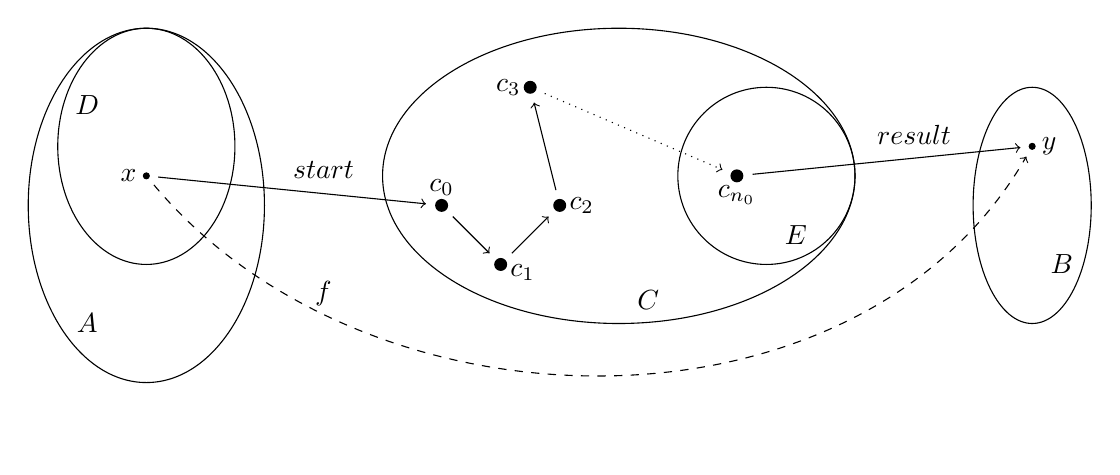
\begin{tikzpicture}[scale=0.75,baseline=(c0)]
\draw (0,0) ellipse (2 and 3);
\draw (8,0.5) ellipse (4 and 2.5);
\draw (15,0) ellipse (1 and 2);
\draw (0,1) ellipse (1.5 and 2);
\draw (10.5,0.5) circle (1.5);
\draw[fill] (0,0.5) coordinate (x) circle (0.05) node[left]{$x$};
\node at(-1,1.7) {$D$};
\node at(-1,-2) {$A$};
\node at(8.5,-1.6) {$C$};
\node at(11,-0.5) {$E$};
\node at(15.5,-1) {$B$};
\node at(3,0.6) {$start$};
\node at(13,1.2) {$result$};
\node at(3,-1.5) {$f$};
\draw[fill] (5,0) coordinate (c0) circle (0.1) node[above]{$c_0$};
\draw[fill] (6,-1) coordinate (c1) circle (0.1) node[right,yshift=-3]{$c_1$};
\draw[fill] (7,0) coordinate (c2) circle (0.1) node[right]{$c_2$};
\draw[fill] (6.5,2) coordinate (c3) circle (0.1) node[left]{$c_3$};
\draw[fill] (10,0.5) coordinate (cn0) circle (0.1) node[below]{$c_{n_0}$};
\draw[fill] (15,1) coordinate (y) circle (0.05) node[right]{$y$};
\draw[shorten <=1.5mm,shorten >=2mm,->] (x) -- (c0);
\draw[shorten <=2mm,shorten >=2mm,->] (c0) -- (c1);
\draw[shorten <=2mm,shorten >=2mm,->] (c1) -- (c2);
\draw[shorten <=2mm,shorten >=2mm,->] (c2) -- (c3);
\draw[dotted,shorten <=2mm,shorten >=2mm,->] (c3) -- (cn0);
\draw[shorten <=2mm,shorten >=1.5mm,->] (cn0) -- (y);
\draw[shorten <=1.5mm, shorten >=1.5mm,dashed,->] (x) to[in=240,out=-50] (y);
%\draw[-] (-2,-1) arc (-130:-50:3);
\end{tikzpicture}    
\end{equation}

% \subsection{Simulacije: intuicija u pozadini dokaza ekvivalentnosti}

Ako sad između istih skupova $A$ i $B$ stavimo još neki drugi skup konfiguracija $C'$, sa svojom funkcijom $nextconf'$ i podskupom završnih konfiguracija $E'$, možemo zamisliti funkciju $start$ kao zadatak $f'$ za taj novi stroj, sa $A':=A$ i $B':=C$. No kako taj stroj zna računati samo funkcije iz $A$ u $B$, moramo prethodno kodirati $C$ nekom funkcijom $Code_1\colon C\to B$. To je zapravo najzanimljiviji dio, jer o njemu ovisi koliko će laki biti kasniji koraci. Dakle $f'=Code_1\circ start$, i kako su te dvije funkcije obično prilično jednostavne, za očekivati je da će $f'$ biti izračunljiva u novom modelu.

\begin{napomena}[{name=[strojevi s apstraktnim stanjima]}]\label{nap:ASM}
Zanimljiv i relativno novi uvid Jurija Gureviča s kraja prošlog stoljeća je da se "univerzalni" skup $C$ može naći u obliku interpretacija za strukture prvog reda. Tada možemo i formalno, koristeći \emph{lokalnost}, definirati što znači "prilično jednostavna" funkcija: to je ona koja ovisi o konačno mnogo "elemenata" (vrijednosti zatvorenih terma) u interpretaciji. Taj uvid vodi na formalizaciju \emph{strojeva s apstraktnim stanjima} (ASM), koji u nekom smislu predstavljaju "univerzalnu podlogu" za opis algoritama. Lijep uvod u ASM-teoriju, pisan specifično za računarce, može se naći u~\cite{huggins}.
\end{napomena}

Analogni postupak možemo napraviti za $result$, samo s druge strane; i za $nextconf$, kodiranjem s obje strane. Svaka od tako dobivenih funkcija sama za sebe je dovoljno jednostavna (u smislu prethodne napomene) da je iz\-ra\-čun\-lji\-va u novom modelu.

No to zapravo znači da sustav $C'$ može simulirati svaki korak $\mathcal A$-izračunavanja, pa može simulirati i čitavo to izračunavanje. Samo treba unutar tog sustava imati neki način za:
\begin{itemize}
    \item određivanje $c_n$ iz $n$, iteriranjem funkcije $nextconf$ (ograničena petlja);
    \item otkrivanje $n_0$ ako postoji (neograničena petlja); te
    \item dobivanje funkcije $f$ iz tako dobivene funkcije $c_0\mapsto c_{n_0}$, $start$ i $result$ (slijed).
\end{itemize}

Sada jasnije vidimo i zašto je skup $\N$ "poseban": dok $A$, $B$ i $C$ mogu biti svakakvi prebrojivi skupovi, domena izračunavanja (kao niza konfiguracija) mora biti $\N$. Drugim riječima, za bilo kakvo metaprogramiranje (koje je nužno za univerzalnu funkciju) model u kojem radimo, pored reprezentacije ulaznih i izlaznih podataka, mora moći reprezentirati i prirodne brojeve. Onda je svakako najjednostavnije da ulazni i izlazni podaci također budu prirodni brojevi.

Odgovarajućim kodiranjima možemo dobiti i simulaciju za promijenjene skupove $A'$ i $B'$ --- baš kao što smo to već činili kad je jedan od tih skupova, ili oba, bio $C$ (za funkcije $start$, $result$ i $nextconf$).

Zato nije čudno da sve formalizacije algoritama koje se mogu svesti na paradigmu shematski prikazanu u~\eqref{dia:alg}, mogu simulirati jedna drugu. Možemo ići toliko daleko da kažemo da je \textbf{prikazivost u obliku takve sheme ono esencijalno što algoritme čini algoritmima}.

Iako je to intuitivno jasno, iz toga nipošto ne slijedi da je svaki model jednostavno svesti na tu shemu. Recimo, možete se zabaviti pokušavajući konstruirati stroj --- sustav $(C,start,nextconf,E,result)$ --- koji računa parcijalno rekurzivne funkcije zadane simboličkim definicijama (ili još kompliciranije, točkovnim definicijama). Koliko god taj zadatak bio prekriven debelim slojem tehničkih detalja, vjerojatno ćete se složiti da su to \emph{samo} tehnički detalji --- izuzetno biste se iznenadili da nekim slučajem ispadne da je takav stroj nemoguće konstruirati, zar ne? Upravo ta intuicija je ono što opravdava Church--\!Turingovu tezu.

\subsection{Fiksiranje pojma algoritma}

Zapravo, postoji širok (i višedimenzijski!) "prostor kompromisa" (\emph{tradeoffs}) prilikom dizajniranja takvih sustava. Na jednom kraju su sasvim jednostavni "konkretni" sustavi za koje je odmah jasno što su konfiguracije i kako je funkcija $nextconf$ zadana --- recimo, RAM-strojevi. Na drugom kraju su sasvim apstraktni sustavi kod kojih su tri nabrojene esencijalne operacije (ograničena i neograničena petlja, te slijed) aksiomatski propisane --- recimo, u sustavu parcijalno rekurzivnih funkcija, redom kao primitivna rekurzija, minimizacija i kompozicija.

Osim s obzirom na apstraktnost, možemo gledati i kompromise s obzirom na druge dimenzije: smanjivanje broja različitih koncepata u sustavu (\emph{Occamova britva}) vodi na sustave u kojima je gotovo sve prikazano prirodnim brojevima (jer, kao što smo rekli, prirodne brojeve moramo imati za reprezentaciju samog izračunavanja). Intuitivna bliskost onom što doista činimo kad provodimo algoritam vodi na sustave koji emuliraju naše stanje uma, i mentalne operacije (pamćenja simbola i jednostavnih odluka na nižoj razini, ili uočavanja obrazaca i vizualizacije njihove supstitucije na višoj razini apstrakcije) --- kao što su jezični modeli izračunavanja.
\begin{equation}\label{eq:vrste-alg}
    \begin{tabular}{c@{\quad}|@{\quad}cc}
        algoritam & konkretni (imperativni) & apstraktni (funkcijski)\\\hline
     jezični (praktični) & Turingov stroj & $\lambda$-račun\\
     brojevni (teorijski) & RAM-stroj & parcijalna rekurzivnost
    \end{tabular}
\end{equation}

Naravno, tablica~\eqref{eq:vrste-alg} je vrlo pojednostavljena --- em postoji puno više dimenzija po kojima možemo uspoređivati algoritamske formalizme (strukturalnost, primjenjivost na stvarne probleme, entropija, količina pretpostavljenog znanja,~\ldots), em prikazane dimenzije nisu binarne. Pored jezičnog i brojevnog modela postoje razni drugi, recimo geometrijski (Wangove domine) ili algebarski (diofantski skupovi), pa čak i topološki (homotopska teorija tipova); dok je konkretno--apstraktno "podjela" zapravo spektar duž kojeg se mogu smjestiti razni koncepti. Recimo, makro-stroj je mrvicu apstraktniji od RAM-stroja, dok je logika prvog reda malo konkretnija od $\lambda$-računa. Čak ni sustavi koje smo obradili nisu ekstremi na tom spektru: postoje i sustavi poput G\"odel--Herbrandovih jednadžbi, koji su još apstraktniji od parcijalne rekurzivnosti, kao i Minskijevi brojači (\emph{counter machines}) koji su još konkretniji od RAM-strojeva. Već smo spomenuli ASM u napomeni~\ref{nap:ASM} --- taj model se proteže duž cijelog spektra konkretno--apstraktno, jer je njegova osnovna odlika da hvata algoritme na njihovoj \textbf{prirodnoj razini apstrakcije}, koja god ona bila.

Ono što je sada bitno je da između ćelija takve tablice možemo slobodno "putovati" kako nam je drago, dok imamo odgovarajuće teoreme ekvivalencije. Za pojedini redak (vrstu ulaznih odnosno izlaznih podataka) to se može sasvim formalizirati, u smislu da su izračunljive funkcije doslovno iste bez obzira na to koji stupac odaberemo. Za različite retke, moramo se dogovoriti oko prirodnog kodiranja, no to je najčešće prilično jednostavno i dosta robusno s obzirom na tehničke detalje (recimo, zapis broja u bazi je vrlo prirodna veza brojevnog i jezičnog modela, i pritom za samu izračunljivost čak nije bitno --- iako za složenost jest --- odaberemo li unarni zapis ili zapis u bazi $b\ge2$).

%\textbf{Church--\!Turingova teza}
\begin{ctteza}
Svaka dovoljno općenita formalizacija pojma algoritma na istoj vrsti podataka ra\-ču\-na iste funkcije, a na različitim vrstama podataka računa funkcije koje su vezane prirodnim kodiranjima između tih vrsta podataka. To su upravo \emph{izračunljive} funkcije, one za koje u intuitivnom smislu postoje algoritmi.
\end{ctteza}

Teoremi ekvivalencije mogu se sada izreći kao: sve ćelije u tablici~\eqref{eq:vrste-alg} jesu dovoljno općenite formalizacije pojma algoritma. (Nismo definirali $\lambda$-račun, ali i za njega vrijedi teorem ekvivalencije. Zainteresirani čitatelj može naći detalje u~\cite{lovnicki}.)

Povijesno, Alonzo Church je autor teze, i prvi koji je primijetio da je teza potrebna kako bi se dokazali rezultati o nepostojanju algoritma. Ipak, njegova formalizacija ($\lambda$-račun) bila je preapstraktna da bi zadovoljila vodeće eksperte za izračunljivost toga doba. To je između ostalog potaklo Turinga na detaljnu analizu intuitivnog pojma algoritma, te je njegova formalizacija, kad je dokazana ekvivalentnom ostalima do tad poznatima, vrlo brzo prihvaćena kao "mjera" (\!\emph{Turing completeness}) pomoću koje se procjenjuju algoritamski sustavi (primjerice, programski jezici) sve do danas.

\begin{quote}
    Church: ``\!{\emph{Turing's notion made the identification with effectiveness in the ordinary (not explicitly defined) sense evident immediately.}}''
    
    G\"odel: ``\!{\emph{The correct definition of mechanical computability was established beyond any doubt by Turing.}}''
    %Dodati Trahtenbrota miracle
\end{quote}

Church--\!Turingova teza nije uobličena kao teorem, pa čak niti kao tvrdnja koju bi se u principu moglo dokazati. U moderno vrijeme postoje i inicijative~\cite{soare} da se ona uobliči kao \emph{definicija}, fiksirajući jedan koncept izračuljivosti.

\begin{definicija}[Soare]\label{def:izr}
Za jezičnu funkciju $\varphi$ kažemo da je \emph{izračunljiva} ako postoji Turingov stroj koji je računa.
Za brojevnu funkciju $f$ kažemo da je \emph{izračunljiva} ako je njena binarna reprezentacija $\beta f$ izračunljiva.
%Umjesto "$f$ je izračunljiva" govorimo još "postoji algoritam za $f$".
\end{definicija}

U tom svjetlu, teoremi ekvivalencije bili bi \emph{karakterizacije} upravo definiranog pojma izračunljivosti. Ipak, u uvodnom kursu je vjerojatno bolje vidjeti interakciju raznih formalizacija, prije nego što se jedna od njih odabere kao definicija. Iako je modernom fizičaru sasvim prirodna definicija "metar je udaljenost koju svjetlost u vakuumu prijeđe za $\frac{1}{299\,792\,458}\,s$", to nije dobra definicija u osnovnoškolskoj nastavi fizike, jer pretpostavlja puno znanja i iskustva o prirodi svjetlosti, inercijalnim sustavima, i teoriji relativnosti. Bez tog znanja definicija se također može prihvatiti, ali djeluje forsirano. Autorovo mišljenje je da bi jednako tako djelovala i definicija~\ref{def:izr} prije dokaza teorema ekvivalencije. Smijete se usprotiviti tom uvjerenju --- ono nije matematičko, već psihološko.

\section{Neizračunljive funkcije}

Intuitivni pojam izračunljivog kao "onog za što postoji algoritam", zajedno s Church--\!Turingovom tezom, napokon daju mogućnost da dokažemo da za neke probleme ne postoje algoritmi. To ćemo učiniti dokazom da neka funkcija $g$ nije parcijalno rekurzivna --- tada po teoremu ekvivalencije njena binarna reprezentacija nije Turing-izračunljiva, po definiciji~\ref{def:izr} $g$ nije izračunljiva, te možemo reći da za nju ne postoji algoritam.

Doduše, obično se problemi za koje se utvrđuje postojanje algoritma iskazuju u obliku \emph{problema odluke}: za dani skup $A$ i njegov podskup $D$, postoji li algoritam koji odlučuje, za proizvoljni $x\in A$, je li $x\in D$? Jednom kada imamo kodiranje $\N A$ skupa $A$, to gledamo kao pitanje izračunljivosti skupa (jednomjesne relacije) $\N A[D]\subseteq\N$, odnosno njene karakteristične funkcije $\chi_{\N A[D]}$. Sve te ideje smo već vidjeli (za $A:=\Sigma^*$) kad smo promatrali odlučive jezike.

\begin{definicija}[{name=[odlučivost problema]}]
Za brojevni problem $D$ kažemo da je \emph{odlučiv} ako je njegova karakteristična funkcija $\chi_D$ rekurzivna. Za problem $D\subseteq A$ takav da postoji prirodno kodiranje $\N A\colon A\to\N$, kažemo da je \emph{odlučiv} ako je brojevni problem $\N A[D]$ odlučiv.
\end{definicija}

"Brojevni problemi" nisu ništa drugo nego relacije, ali postavljeni u obliku pitanja, odnosno ispitivanja nekog svojstva. Recimo, $Halt_2=\dom{\f{comp}_2}^3$ možemo promatrati kao problem "za zadane $x,y,e\in\N$, (postoji li i) stane li program koda $e$ s ulazom $(x,y)$?", odnosno "ima li izraz $\kf{e}(x,y)$ smisla?". Već smo nagovijestili da taj problem nije odlučiv.
Kako bismo to dokazali? Uzmimo za početak nešto lakše. U uvodu smo već spomenuli paradoks sličan Russellovom, koji nastaje ako pretpostavimo da su svi algoritmi totalni: poredali smo sve jednomjesne algoritme u niz $(\mathcal A_n)_n$, i onda za ulaz $n$ primijenili $\mathcal A_n$ na $n$, i vratili sljedbenik izlaznog podatka. Pomoću indeksa možemo to doslovno napraviti.

\begin{definicija}[{name=[Russellova funkcija i Russellov skup]}]
\emph{Russellova funkcija} je jednomjesna funkcija $\f{Russell}^1$ zadana s
\begin{equation}\label{eq:Russelldef}
    \f{Russell}(n):\simeq\f{comp}_1(n,n)+1\text.
\end{equation}
\emph{Russellov skup} je domena Russellove funkcije: $K^1:=\dom{\f{Russell}}$.
\end{definicija}

\begin{korolar}[{name=[parcijalna rekurzivnost Russellove funkcije]}]\label{kor:Russellprek}
Russellova funkcija je parcijalno rekurzivna.
\end{korolar}
\begin{proof}
Točkovna definicija~\eqref{eq:Russelldef} se lako zapiše u simboličkom obliku kao kompozicija $\f{Russell}=\f{Sc}\circ\f{comp}_1\circ(\f I_1^1,\f I_1^1)$, pa tvrdnja slijedi po propoziciji~\ref{prop:compspec}.
\end{proof}

Paradoks iz uvoda sada se može iskazati ovako: imamo algoritam za $\f{Russell}$, ali nijedan algoritam koji računa vrijednosti od $\f{Russell}$ nije totalan. Drugim riječima, Russellova funkcija je izračunljiva, ali ne postoji njeno izračunljivo totalno proširenje.

\begin{lema}[{name=[neproširivost Russellove funkcije do rekurzivne]}]\label{lm:Russellnrek}
Ne postoji rekurzivna funkcija $\f r$ takva da je $\f r|_{K}=\f{Russell}$.
\end{lema}
\begin{proof}
Pretpostavimo da takva funkcija postoji. Tada je ona parcijalno rekurzivna, pa po teoremu ekvivalencije ima indeks, označimo ga s $e$ (vidjeti napomenu~\ref{nap:>1ind}); i totalna je, pa postoji $q:=\f r(e)\in\N$. Sada je sljedbenik od $q$ jednak
\begin{equation}
    1+q=1+\f r(e)=1+\kf e(e)=1+\f{comp}(e,e)\text,
\end{equation}
iz čega slijedi da je $e\in K$ i $\f{Russell}(e)=1+q$. No $\f r(e)=q\not=1+q$, pa $\f r$ ne može biti proširenje od $\f{Russell}$, kontradikcija.
\end{proof}

\begin{teorem}[{name=[nerekurzivnost Russellovog skupa]}]\label{tm:DRnrek}
Russellov skup $K$ nije rekurzivan.
\end{teorem}
\begin{proof}
Pretpostavimo suprotno, i označimo s $\rus:=\{K\colon\f{Russell},\f Z\}$ proširenje Russellove funkcije nulom.
Točkovno, imamo
\begin{equation}
    \rus(n):\simeq
\begin{cases}
\f{Russell}(n),&n\in K\\
0,&\text{inače}
\end{cases}\text.
\end{equation}
Po korolaru~\ref{kor:Russellprek} $\f{Russell}$ je parcijalno rekurzivna, po pretpostavci suprotnog je $K$ rekurzivna relacija, a $\f Z$ je inicijalna pa je trivijalno parcijalno rekurzivna. Prema teoremu~\ref{tm:gprek}, iz toga bi slijedilo da je $\rus$ parcijalno rekurzivna funkcija. 

S druge strane, po definiciji~\ref{def:gr} je $R_0:=K\kompl$, pa je
\begin{equation}
    \dom{\rus}=(\dom{\f Z}\cap R_0)\cup(\dom{\f{Russell}}\cap K)=(\N\cap K\kompl)\cup(K\cap K)=K\kompl\cup K=\N\text,
\end{equation}
dakle $\rus$ je totalna funkcija. To, zajedno s parcijalnom rekurzivnošću, značilo bi da je $\rus$ rekurzivna funkcija, što je u kontradikciji s lemom~\ref{lm:Russellnrek} (očito je $\rus|_{K}=\f{Russell}$).
\end{proof}

Time smo napokon dokazali da postoji izračunljiva funkcija s neizračunljivom domenom, i vidimo u čemu je problem s našom intuicijom: iako proširenje nulom doživljavamo kao trivijalnu operaciju na brojevnoj funkciji, za izračunljivost $\tilde{\f f}$ je potrebno ustanoviti kad ulazni podatak $x$ \emph{nije} u domeni $\dom{\f f}$ (da bismo ga preslikali u $0$) --- a to zapravo zahtijeva da ustanovimo da \emph{nijedna} konfiguracija stroja koji računa $\f f$ na $x$ nije završna. 

To je osnovna nesimetrija u definiciji algoritma: dok je zaustavljanje algoritma moguće karakterizirati neograničenom egzistencijalnom kvantifikacijom (projekcijom), što jest domena izračunljive funkcije (minimizacije), njegovo \emph{nezaustavljanje} nije moguće tako karakterizirati. Ukratko, prirodni brojevi imaju lijepo svojstvo \emph{početne konačnosti}: od svakog prirodnog broja ima konačno mnogo manjih, i ako postoji prirodni broj s nekim svojstvom, prateći sljedbenike od nule stići ćemo do njega u konačno mnogo koraka. S druge strane (doslovno!), prirodnih brojeva ima beskonačno mnogo: od svakog broja ima beskonačno mnogo većih, i ako trebamo ustanoviti da neko svojstvo vrijedi za sve prirodne brojeve, to nikako ne možemo učiniti provjeravajući ih jedan po jedan. Čak i da ih ne provjeravamo po redu, do svakog trenutka smo provjerili samo konačno mnogo njih, te od svih njih postoji najveći, a većih od njega ima jednako mnogo kao i svih prirodnih brojeva.

Naravno, to nije \emph{dokaz} da ne postoji možda neka druga metoda kojom bismo ustanovili da $x\not\in\dom{\f f}$ --- samo pokazuje da stvari nisu tako jednostavne.

\subsection{Svođenje i problemi zaustavljanja}

Problem kojim smo se bavili --- za zadani $n$, je li $n$ u domeni od $\kf n^1$ --- čini se vrlo umjetnim: nije da bismo ikad bili doista zainteresirani za općeniti odgovor na to pitanje. Ipak, jednom kad imamo neki neodlučiv problem, možemo se dočepati i ostalih.

Metoda je ista ona pomoću koje iz već poznatih odlučivih problema (izračunljivih funkcija) dobivamo nove: \emph{svođenje} (redukcija). Ako možemo neku funkciju $f$ svesti na neku drugu $g$ --- napisati $f$ pomoću kompozicije, i eventualno primitivne rekurzije, funkcije $g$ s nekim izračunljivim funcijama, tada znamo da ako je $g$ izračunljiva, tada je i $f$ takva. To smo koristili mnogo puta u funkcijskom programiranju. Doduše, tamo nam je bila bitna primitivna rekurzivnost, pa smo govorili samo o totalnim funkcijama, i primitivna rekurzija je igrala bitnu ulogu. Kad govorimo o (ne)odlučivim problemima, primitivna rekurzivnost postaje luksuz koji si ne možemo uvijek priuštiti, pa ćemo zapravo promatrati samo kompoziciju. Kako se radi o problemima, dakle karakterističnim funkcijama relacija koje su totalne, zbog marljive evaluacije proizlazi da sve funkcije u kompoziciji moraju također biti totalne.

Napomenimo samo da u literaturi postoje razne vrste svođenja problema, pa i općenitih funkcija. Mi ćemo odabrati najjednostavniju koja je dovoljno dobra za naše potrebe.

\begin{definicija}[{name=[svedivost brojevnih relacija]}]
Neka su $k,l\in\N_+$, te $R^k$ i $P^l$ relacije. Kažemo da je $R$ \emph{svediva} na $P$, i pišemo $R\preceq P$, ako postoje rekurzivne funkcije $\f G_1^k$, $\f G_2^k$,~\ldots, $\f G_l^k$ takve da vrijedi $\chi_R=\chi_P\circ(\f G_1,\f G_2,\dotsc,\f G_l)$.
\end{definicija}

Zadnja jednakost se može točkovno zapisati kao $R(\vec x)\Leftrightarrow P\bigl(\f G_1(\vec x),\dotsc,\f G_l(\vec x)\bigr)$. Primijetimo da je to zapravo obična kompozicija $\chi_R=\chi_P\circ G$, samo uzevši u obzir da je kodomena od $G$ jednaka $\N^l$, pa je prikazujemo kroz $l$ koordinatnih funkcija --- što je već standardno kad se o kompoziciji radi.

Također primijetimo da nismo ništa dokomponirali na $\chi_P$ slijeva: nije dozvoljen \emph{post-processing} povratne vrijednosti od $\chi_P$, samo \emph{pre-processing} njenih ulaznih podataka. Kako se radi o karakterističnim funkcijama čije su povratne vrijednosti iz $bool=\{0,1\}$, jedini netrivijalni \emph{post-processing} bi moglo biti negiranje (komplementiranje), ali kako smo upravo vidjeli da komplementiranje općenito nije tako jednostavna operacija na problemima (npr.\ na domenama izračunljivih funkcija, odnosno problemima zaustavljanja), s razlogom ga nećemo htjeti ovdje.

\begin{propozicija}[{name=[refleksivnost i tranzitivnost svedivosti]}]\label{pp:preceqrt}
Relacija $\preceq$ (na skupu $\bigcup_{k\in\N_+}\!\mathcal P(\N^k)$ svih brojevnih relacija) je refleksivna i tranzitivna.
\end{propozicija}
\begin{proof}
Refleksivnost je jednostavna: stavimo $\f G_1:=\f I_1^l$, $\f G_2:=\f I_2^l$,~\ldots, $\f G_l:=\f I_l^l$ (koordinatne funkcije identitete $id_{\N^l}$). Očito je $\chi_P\circ(\f I_1^l,\dotsc,\f I_l^l)=\chi_P$, pa je $P\preceq P$.

Tranzitivnost je kompliciranija, ali samo notacijski, zbog toga što funkcije s više izlaza promatramo kroz koordinatne funkcije. Neka su $k,l,m\in\N_+$, te neka su $R^k$, $Q^m$ i $P^l$ relacije takve da je $R\preceq Q\preceq P$. Prvo svođenje znači da postoje rekurzivne funkcije $\f G_1^k$,~\ldots, $\f G_m^k$ takve da je $\chi_R=\chi_Q\circ(\f G_1,\dotsc,\f G_m)$, dok drugo znači da postoje rekurzivne funkcije $\f H_1^m$,~\ldots, $\f H_l^m$ takve da je $\chi_Q=\chi_P\circ(\f H_1,\dotsc,\f H_l)$. Sada je (možemo pisati jednakosti jer su sve funkcije ili karakteristične ili rekurzivne, dakle totalne, a kompozicija totalnih je totalna po propoziciji~\ref{prop:comptot})
\begin{multline}\label{eq:tranzpreceq}
    \chi_R(\vec x)=\chi_Q\bigl(\f G_1(\vec x),\dotsc,\f G_m(\vec x)\bigr)=\bigl(\chi_P\circ(\f H_1,\dotsc,\f H_l)\bigr)\bigl(\f G_1(\vec x),\dotsc,\f G_m(\vec x)\bigr)=\\
    =\chi_P\bigl(
    \f H_1\bigl(\f G_1(\vec x),\dotsc,\f G_m(\vec x)\bigr),\dotsc,
    \f H_l\bigl(\f G_1(\vec x),\dotsc,\f G_m(\vec x)\bigr)
    \bigr)=\\
    =\chi_P\bigl(
    \bigl(\f H_1\circ(\f G_1,\dotsc,\f G_m)\bigr)(\vec x),\dotsc,
    \bigl(\f H_l\circ(\f G_1,\dotsc,\f G_m)\bigr)(\vec x)\bigr)=\\
    =\bigl(\chi_P\circ\bigl(\f H_1\circ(\f G_1,\dotsc,\f G_m),\dotsc,\f H_l\circ(\f G_1,\dotsc,\f G_m)\bigr)\bigr)(\vec x)\text,
\end{multline}
dakle ako za svaki $i\in[1..l]$ definiramo $\f F_i:=\f H_i\circ(\f G_1,\dotsc,\f G_m)$, tada je svaka $\f F_i$ rekurzivna po lemi~\ref{lm:comprek}. Sada~\eqref{eq:tranzpreceq} možemo zapisati kao $\chi_R=\chi_P\circ(\f F_1,\dotsc,\f F_l)$, odakle slijedi $R\preceq P$.
\end{proof}

Relacija $R\preceq P$ znači da ako imamo algoritam za rješavanje problema $P$, pomoću njega možemo riješiti i problem $R$. Intuitivno, $R$ je "barem toliko odlučiv" koliko i $P$.

\begin{propozicija}[{name=[svedivost čuva rekurzivnost]}]\label{pp:rek<rek}
Relacija svediva na rekurzivnu relaciju je i sama rekurzivna.
\end{propozicija}
\begin{proof}
Neka su $k,l\in\N_+$, te $R^k$ relacija i $\f P^l$ rekurzivna relacija, takve da je $R\preceq\f P$. To znači $\chi_R=\chi_{\f P}\circ(\f G_1,\dotsc,\f G_l)$, a rekurzivnost od $\f P$ znači da je $\chi_{\f P}$ rekurzivna, pa je po lemi~\ref{lm:comprek} i $\chi_R$ rekurzivna, odnosno $R$ je rekurzivna.
\end{proof}

\begin{korolar}[{name=[inverz svedivosti čuva neodlučivost]}]\label{kor:nrek<nrek}
Ako je $R\preceq P$ i $R$ nije odlučiv, tada ni $P$ nije odlučiv.
\end{korolar}
\begin{proof}
Ovo je samo kontrapozicija propozicije~\ref{pp:rek<rek}, iskazana jezikom problema.
\end{proof}

% \section{Problemi zaustavljanja}

Korolar~\ref{kor:nrek<nrek}, kao što smo već nagovijestili, pruža način da pomoću jednog neodlučivog problema dođemo do ostalih.

\begin{propozicija}[{name=[neodlučivost problema zaustavljanja za RAM-strojeve]}]\label{pp:Haltnodl}
Problemi $Halt_1$ i $HALT$ nisu odlučivi.
\end{propozicija}
\begin{proof}
Tvrdimo da vrijedi $K(n)\Leftrightarrow Halt_1(n,n)$. Doista,
\begin{multline}
    K=\dom{\f{Russell}}=\dom{\f{Sc}\,\circ\,\f{comp_1}\circ(\f I_1^1,\f I_1^1)}=\dom{\f{comp}_1\circ(\f I_1^1,\f I_1^1)}=\\
    =\left\{n\;\middle\vert\;\bigl(\f I_1^1(n),\f I_1^1(n)\bigr)\in\dom{\f{comp}_1}\right\}
    =\{n\mid(n,n)\in Halt_1\}\text,
\end{multline}
gdje smo koristili definiciju~\eqref{eq:domkomp}, i njenu laganu posljedicu da je $\dom{F\circ G}=\dom G$ ako je $F$ totalna. Iz toga slijedi $K\preceq Halt_1$, pa je $Halt_1$ neodlučiv po korolaru~\ref{kor:nrek<nrek} i teoremu~\ref{tm:DRnrek}.

Slično, po definiciji iz korolara~\ref{kor:funHaltTk}, vrijedi $Halt_1(x,e)\Leftrightarrow HALT(\kr x,e)$, a funkcija $\f{Code}^1$ je (primitivno) rekurzivna, te je $Halt_1\!\preceq HALT$, iz čega je i $HALT$ neodlučiv.
\end{proof}

U literaturi se $Halt_1$ odnosno $HALT$ (kako gdje) zove \emph{halting problem} (problem zaustavljanja), jer postavlja pitanje stane li određeno izračunavanje (zadano pomoću RAM-programa i ulaza za njega). Mogli bismo dokazati i neodlučivost problema $Halt_k$ za $k\ge 2$ (pokušajte formalno dokazati svođenje $Halt_1(x,e)\Leftrightarrow Halt_k(x,0,0,\dotsc,0,e)$), ali to će lako slijediti jednom kad dokažemo teorem o parametru.

Dakle, ono što zasad znamo, po Church--\!Turingovoj tezi, je da ne postoji algoritam koji bi za svaki par RAM-stroja $P$ i ulaza $u$ za njega odlučivao stane li $P$-izračunavanje s $u$ --- odnosno, za svaki algoritam $\mathcal A$ postoji RAM-program $P$ i prirodni broj $u$ takav da $\mathcal A$ ne daje ispravan odgovor na pitanje stane li $P$-izračunavanje s $u$. Ali znamo i više: možemo postići da $P$ ne ovisi o $\mathcal A$. To je u skladu s univerzalnošću: postoji "najkompliciraniji" RAM-stroj, čiji je problem zaustavljanja najteži.

\begin{korolar}[{name=[neodlučivost problema zaustavljanja za jedan fiksni RAM-stroj]}]\label{kor:RAMhaltnodl}
Postoji RAM-program $P_0$, takav da nijedan algoritam ne može točno odrediti, za svaki $u\in\N$, stane li $P_0$-izračunavanje s $u$.
\end{korolar}
\begin{proof}
%Jednostavno kompajliramo (teorem~\ref{tm:pir}) simboličku definiciju funkcije $\f{Russell}$ koju smo dobili u dokazu korolara~\ref{kor:Russellprek}. Tako dobijemo RAM-program $P_0$, za koji po definiciji~\ref{def:compute} vrijedi: za svaki $t\in\N$, $P_0$-izračunavanje s $t$ stane ako i samo ako je $t\in K$.
Po korolaru~\ref{kor:Russellprek}, Russellova funkcija je parcijalno rekurzivna. Po teoremu~\ref{tm:pir}, ona je i RAM-izračunljiva. Označimo s $P_0$ jedan RAM-program koji je računa. Po definiciji~\ref{def:compute}, za svaki $u\in\N$, $P_0$-izračunavanje s $u$ stane ako i samo ako je $u\in K$.

Kad bi postojao algoritam za odlučivanje problema zaustavljanja $P_0$-izračunavanja s proizvoljnim $u$, po Church--\!Turingovoj tezi $K$ bi bio odlučiv problem, što je u kontradikciji s teoremom~\ref{tm:DRnrek}.
\end{proof}

\begin{lema}[{name=[neodlučivost problema zaustavljanja za jedan fiksni Turingov stroj]}]\label{lm:THaltnodl}
Postoji Turingov stroj $\mathcal T_0$ nad unarnom abecedom $\Sigma_{\t\textbullet}=\{\t\textbullet\}$, takav da nijedan algoritam ne može točno odrediti, za svaku riječ $w\in\t\textbullet^*$\!, stane li $\mathcal T_0$-izračunavanje s $w$.
\end{lema}
\begin{proof}
Po korolaru~\ref{kor:peuf}, jezična funkcija $\rho:=\t\textbullet\f{Russell}$ je Turing-izračunljiva, te vrijedi
\begin{equation}\label{eq:rhoRussell}
    \rho(\t\textbullet^t)\simeq\t\textbullet^{\f{Russell}(t)}\text.
\end{equation}
To znači da za $\mathcal T_0$ možemo uzeti Turingov stroj koji računa $\rho$. Očito $\mathcal T_0$ jest nad unarnom abecedom, i stane točno za riječi oblika $\t\textbullet^t$ za $t\in K$.

Sad, kada bi postojao algoritam koji bi za svaku riječ nad $\Sigma_{\t\textbullet}$ odlučivao hoće li $\mathcal T_0$-izračunavanje s njome stati, pomoću njega bismo mogli odlučiti $K$, sljedećim algoritmom: za ulaz $u\in\N$, konstruiramo riječ $\t\textbullet^u$, i vratimo stane li $\mathcal T_0$-izračunavanje s njom. Po definiciji~\ref{def:Tcomputefi}, to će biti ako i samo ako je $\t\textbullet^u\in\dom\rho$, što će prema definiciji unarne reprezentacije biti ako i samo ako je $u\in K$. Po Church--\!Turingovoj tezi, to bi značilo da je $K$ rekurzivna, što je u kontradikciji s teoremom~\ref{tm:DRnrek}.
\end{proof}

\begin{propozicija}[Neodlučivost problema zaustavljanja za Turingove strojeve]
Za svaku abecedu $\Sigma$ postoji Turingov stroj nad njom, čiji je problem zaustavljanja neodlučiv.
\end{propozicija}
\begin{proof}
Ako je $\t\textbullet\;\raisebox{1.1pt}{$\in$}\;\Sigma$, možemo direktno primijeniti lemu~\ref{lm:THaltnodl}, na Turingov stroj $\mathcal T_0$ s abecedom $\Sigma$. Kad bi postojao algoritam koji za svaku riječ $w\in\Sigma^*$ točno određuje stane li $\mathcal T_0$-izračunavanje s $w$, to bi specijalno moralo vrijediti za sve $w\in\t\textbullet^*\subseteq\Sigma^*$, što je u kontradikciji s lemom~\ref{lm:THaltnodl}.

Ako pak $\t\textbullet\;\raisebox{1.1pt}{$\not\in$}\;\Sigma$, uzmimo neki konkretni znak $\alpha\in\Sigma$ (po definiciji abecede je $\Sigma\not=\emptyset$, pa $\alpha$ postoji), i \emph{zamijenimo} ga s \t\textbullet: gledamo Turingov stroj $\mathcal T_0'$ koji je kao $\mathcal T_0$ iz prethodnog odlomka, osim što umjesto \t\textbullet\ ima $\alpha$ --- kako u $\Sigma$, tako i u $\Gamma$ i u svim prijelazima od $\delta$. S obzirom na to da znakovi radne abecede nemaju nikakvu imanentnu semantiku (osim praznine, ali za to pogledajte sljedeći odlomak), $\mathcal T_0'$-izračunavanje s $\alpha^u$ stane ako i samo ako $\mathcal T_0$-izračunavanje s $\t\textbullet^u$ stane --- pa kad bi neki algoritam za svaku $w\in\Sigma^*$ točno određivao stane li $\mathcal T_0'$-izračunavanje s $w$, tada bi to specijalno vrijedilo i za sve riječi oblika $\alpha^u,u\in\N$, pa bismo opet imali kontradikciju s neodlučivošću od $K$ kao u prethodnom odlomku.

Jedan detalj još moramo uzeti u obzir: što ako je praznina stroja $\mathcal T_0$ upravo \t\textbullet? Tada ona po definiciji nije u $\Sigma$, ali je ne možemo jednostavno zamijeniti s $\alpha$ jer $\alpha$ jest u $\Sigma$. U tom slučaju odaberemo neki novi znak $\beta\not\in\Gamma$, proglasimo ga prazninom, i \t\textbullet\ zamijenimo s $\beta$ u $\Gamma$ i $\delta$. Nakon toga primijenimo postupak iz prethodnog odlomka.
\end{proof}

\section{Neodlučivost u logici prvog reda}

%Jedan od najvažnijih rezultata o neodlučivosti je svakako Churchov teorem o neodlučivosti logike prvog reda. 
U uvodnom kursu matematičke logike obično se za logiku sudova dokažu teoremi adekvatnosti i potpunosti (koji povezuju sintaksni pojam dokazivosti sa semantičkim pojmom valjanosti), te se navedu neki sustavi (npr.\ glavni test) koji u potpunosti određuju je li neka formula valjana ili nije. Drugim riječima, postoji algoritam za utvrđivanje valjanosti. Postoji li \emph{polinomni} algoritam za to, je zanimljivije pitanje i vodi na slavni milijun dolara vrijedan problem $P\stackrel?=NP$, ali barem znamo da je valjanost odlučiva. Štoviše, nije prevelik problem (i dobra je vježba), koristeći kodiranje opisano u primjeru~\ref{pr:lskod}, formalno dokazati da je skup $\f{PValid}\subset\f{PF}$, svih kodova valjanih formula logike sudova, primitivno rekurzivan. Praktički jedino na što treba misliti je da je ne možemo kodirati (totalne) interpretacije jer ih ima neprebrojivo mnogo, ali parcijalne interpretacije (s konačnom domenom) možemo.

U logici prvog reda, također vrijede teoremi adekvatnosti i potpunosti (dakle, postoji dokaz za formulu $\phi$ koji koristi samo aksiome i pravila zaključivanja logike prvog reda, ako i samo ako je $\phi$ istinita u svim $\sigma$-strukturama prvog reda, gdje je $\sigma$ signatura koja sadrži sve nelogičke simbole u $\phi$), i također imamo glavni test, i znamo da je korektan (odgovor koji dade je uvijek točan), ali nije totalan --- mogu postojati beskonačne grane, u kojima algoritam ne daje odgovor. I to nije nedostatak specifičnog algoritma: jedan od prvih i najvažnijih rezultata o neodlučivosti je Churchov teorem da \textbf{problem valjanosti za logiku prvog reda nije odlučiv}. Skraćeno kažemo "logika prvog reda nije odlučiva", i doista, valjanost tu nije esencijalna. Ekvivalentno možemo promatrati probleme ispunjivosti, oborivosti, proturječnosti, ili čak zaključivanja (logičke posljedice iz konačnog skupa formula). Mi ćemo promatrati problem koji prirodno ima oblik problema zaključivanja, pa je prirodno usredotočiti se na njegovu vezu s problemom valjanosti.

\begin{definicija}[{name=[problem valjanosti i problem zaključivanja]}]
Označimo s $F1$ skup svih formula nad jezikom logike prvog reda.

\emph{Problem valjanosti} pita: za proizvoljnu formulu $\phi\in F1$, je li $\phi$ valjana?

\emph{Problem zaključivanja} pita: za proizvoljni $k\in\N$, za proizvoljne $\phi_1,\phi_2,\dotsc,\phi_k\in F1$, za proizvoljnu $\phi\in F1$, je li $\phi$ logička posljedica skupa $\{\phi_1,\dotsc,\phi_k\}$?
\end{definicija}

\begin{propozicija}[{name=[međusobna svedivost valjanosti i zaključivanja]}]\label{pp:valj<>zaklj}
Problemi valjanosti i zaključivanja svedivi su jedan na drugi.
\end{propozicija}
\begin{proof}
Možemo samo neformalno pričati o svođenju, jer još nismo precizirali abecedu i jezik logike prvog reda. Taj jezik jest detaljno prikazan u~\cite{skr:VukML}, ali nad beskonačnom abecedom, što nije dovoljno dobro za naše potrebe (pokušajte otkriti na kojim smo sve mjestima dosad koristili konačnost abecede). Uz nekoliko jednostavnih modifikacija, prilagodit ćemo taj jezik teoriji formalnih jezika, ali zasad samo opišimo ideje.

U jednom smjeru, zamislimo da imamo instancu problema valjanosti, i algoritam ("crnu kutiju") za odluku problema zaključivanja. Pitamo se što uvrstiti u taj algoritam, da dobijemo odgovor na pitanje valjanosti. Naravno,  ako zadana instanca pita je li $\phi$ valjana, odgovor na to pitanje je isti kao i na pitanje je li $\phi$ posljedica praznog skupa formula --- dakle stavimo $k=0$ (i ne moramo zadavati formule $\phi_i$ jer ih nema).

U drugom smjeru je malo zanimljivije. Pretpostavimo da imamo algoritam za utvrđivanje valjanosti, i da su nam zadane formule $\phi_1$, $\phi_2$,~\ldots, $\phi_k$ i $\phi$, te se pitamo je li $\phi$ logička posljedica ovih prethodnih. Svođenje možemo opisati indukcijom po $k\in\N$. Baza je ista kao gore: za $k=0$, zapravo se pitamo je li $\phi$ valjana. Pretpostavimo da je problem zaključivanja za $k=l$ svediv na problem valjanosti, i pogledajmo problem zaključivanja za $k=l+1$. Također, zbog jakog teorema potpunosti svejedno je koristimo li relaciju logičke posljedice $\models$ ili izvedivosti $\vdash$.

Ako je zadnja premisa $\phi_{l+1}$ \emph{rečenica} (zatvorena formula, bez slobodnih varijabli), možemo primijeniti teorem dedukcije (za jedan smjer --- drugi smjer je trivijalan pomoću pravila zaključivanja \emph{modus ponens}):
\begin{equation}\label{eq:prebaci}
\phi_1,\dotsc,\phi_l,\phi_{l+1}\vdash\phi\text{\quad ako i samo ako\quad}
\phi_1,\dotsc,\phi_l\vdash(\phi_{l+1}\to\phi)\text,
\end{equation}
zbog kojeg je problem zaključivanja s $l+1$ premisom svediv na problem zaključivanja s $l$ premisa, a onda po pretpostavci indukcije i po tranzitivnosti na problem valjanosti.

Ako formula $\phi_{l+1}$ nije rečenica, umjesto nje možemo promotriti njeno \emph{univerzalno zatvorenje} $\overline{\phi_{l+1}}$, dobiveno univerzalnim kvantificiranjem svih slobodnih varijabli u $\phi_{l+1}$. Lako se vidi da $\mathfrak N\models\phi_{l+1}$ ako i samo ako $\mathfrak N\models\overline{\phi_{l+1}}$, dakle odgovor na problem zaključivanja neće se promijeniti, a $\overline{\phi_{l+1}}$ jest rečenica, pa možemo primijeniti teorem dedukcije kao u prethodnom odlomku.
\end{proof}
Za dovršetak odnosno formalizaciju dokaza još bi trebalo vidjeti da je funkcija koja preslikava $\bigl(\phi_1,\dotsc,\phi_l,\phi_{l+1},\phi\bigr)$ u $\bigl(\phi_1,\dotsc,\phi_l,(\overline{\phi_{l+1}}\to\phi)\bigr)$ rekurzivna (zadana s $l+1$ koordinatnih funkcija na kodovima, prvih $l$ od kojih su inicijalne), što zasad ne možemo jer nemamo kodiranje $F1$ --- ali je intuitivno jasno da to možemo učiniti samo mehaničkim manipulacijama simbolima od kojih se formule sastoje.

\subsection{Reprezentacija RAM-konfiguracija formulama prvog reda}

Osnovna ideja dokaza Churchovog teorema je svesti problem zaustavljanja za RAM-strojeve na problem zaključivanja. Iz toga će onda Churchov teorem odmah slijediti po propoziciji~\ref{pp:Haltnodl} i korolaru~\ref{kor:nrek<nrek}.

Dakle, neka su $k\in\N_+$, $P\in\mathcal Prog$, te $\vec u\in\N^k$ (u logici prvog reda obično individualne varijable označavamo s $x_i$, pa ćemo ovdje koristiti $u_i$ kao uobičajenu oznaku za ulazne podatke). Trebamo konstruirati skup formula $\Gamma$ i formulu $\zeta$, koji ovise o $P$ i $\vec u$, tako da $P$-izračunavanje s $\vec u$ stane ako i samo ako vrijedi $\Gamma\models\zeta$. Štoviše, zbog korolara~\ref{kor:RAMhaltnodl}, zapravo možemo cijelu konstrukciju provesti za fiksni $P$ (i za $k=1$), pa ga nećemo pisati (iako smo svjesni da će $\Gamma$ i $\zeta$ ovisiti o $P$).

Logičko zaključivanje je, u osnovi, traženje "puta" od premisa do zaključka, i osnovni razlog zašto je to težak problem je što znamo da put (\emph{izvod}) postoji kad ga nađemo, ali dok ga nismo našli, ne znamo je li to zato što ne postoji, ili samo nismo tražili dovoljno dugo. To vrlo podsjeća na traženje "puta" od početne do završne konfiguracije pri rješavanju problema zaustavljanja --- možemo li nekako formalizirati tu vezu?

Očito, u tom smislu, u $\Gamma$ bi se trebala nalaziti neka formula $\pi_{\vec u}$ koja opisuje početnu konfiguraciju s ulazom $\vec u$, a $\zeta$ bi trebala biti formula koja opisuje neku (bilo koju) završnu konfiguraciju --- kako nas ne zanima rezultat izračunavanja, nego samo zaustavljanje, $\zeta$ očito može biti egzistencijalno kvantificirana po stanju registara, i samo fiksirati vrijednost programskog brojača, a onda ne mora ovisiti o $\vec u$.

U tom smislu, instrukcije programa $P$ mogli bismo shvatiti kao pravila zaključivanja --- recimo, $3.\;\incr1$ kaže da iz formule koja predstavlja konfiguraciju $(x,y,\vec z,0,\dotsc,3)$ možemo izvesti formulu koja predstavlja konfiguraciju $(x,y+1,\vec z,0,\dotsc,4)$, za sve $x$, $y$ i $\vec z$ --- ali s time postoji jedan bitan problem: logika prvog reda ne dopušta nam imati vlastita (nelogička) pravila zaključivanja, možemo imati samo \emph{modus ponens} i generalizaciju. Srećom, \emph{modus ponens} je vrlo općenito pravilo, koje može simulirati ostala pravila putem odgovarajućih nelogičkih aksioma --- primjerice, ako bismo htjeli imati pravilo kojim iz $A$ i $B$ izvodimo $C$, dovoljno je u nelogičke aksiome dodati formulu $\bigl(A\to(B\to C)\bigr)$. Tada možemo iz tog aksioma i $A$ izvesti $(B\to C)$, pa onda iz toga i $B$ izvesti $C$, koristeći samo \emph{modus ponens}.

Taj pristup ćemo koristiti ovdje, odnosno u $\Gamma$ ćemo imati po jednu formulu $\iota_i$ za svaku instrukciju programa $P$ (s rednim brojem $i$). Još je preostalo objasniti što ćemo s ovim trotočkama u konfiguracijama (odnosno kako reprezentirati konačni nosač), i što s aritmetičkim operacijama ($+$ za \inc, $-$ za \dec).

Konfiguracije prikazujemo određenim atomarnim formulama. Sadržaj programskog brojača, budući da je jedan od konačno mnogo njih (za fiksan RAM-program $P$), kodirat ćemo statički, kroz supskript relacijskog simbola odgovarajuće atomarne formule --- a sadržaj pojedinih registara preko terma u toj formuli. Ipak, kako svaka (atomarna) formula može imati samo konačno mnogo terma, morat ćemo se ograničiti samo na relevantne registre.

Aritmetiku bismo mogli prikazati nekom 
varijantom Peanove aritmetike, ali zapravo možemo i lakše: budući da je sve što nam treba sljedbenik i prethodnik, dovoljno je imati jedan konstantski simbol (koji predstavlja nulu) i jedan jednomjesni funkcijski simbol (koji predstavlja funkciju sljedbenik). Zatvoreni termi onda na očit način predstavljaju prirodne brojeve: broj $u$ je predstavljen termom koji predstavlja $u$-struku primjenu tog funkcijskog simbola na taj konstantski simbol.

Napomenimo samo da ne promatramo logiku prvog reda s jednakošću --- nećemo uopće imati potrebu promatrati jednakost, a kamoli kao relacijski simbol s nekim posebnim svojstvima. Usporedba s nulom za instrukciju \dec\ bit će sintaksna.

Vrijeme je da počnemo pričati formalnije: krenimo od RAM-programa $P$, i mjesnosti $k$ (drugim riječima, od RAM-algoritma $P^k$). Označimo s $n:=n_P$ duljinu programa $P$, i s $m:=m_{P^k}$ širinu algoritma $P^k$. Signatura $\sigma$, nad kojom ćemo graditi formule za naš problem zaključivanja, imat će:
\begin{itemize}
    \item jedan konstantski simbol $\mathsf 0$;
    \item jedan jednomjesni funkcijski simbol $\mathsf s$;
    \item $n+1$ $m$-mjesnih relacijskih simbola $R_0^m$,~$R_1^m$,~\ldots,~$R_n^m$.
\end{itemize}

Za svaki $u\in\N$, zatvoreni term $\mathsf s(\mathsf s(\dotsb(\mathsf s(\mathsf0))\dotsb))$ u kojem ima $u$ pojava funkcijskog simbola $\mathsf s$, skraćeno označavamo s $\overline u$ --- dakle $\overline 0=\mathsf 0$, $\overline 1=\mathsf s(\mathsf0)$, $\overline 2=\mathsf s\bigl(\mathsf s(\mathsf0)\bigr)$ itd. Za proizvoljni $\vec u=(u_1,u_2,\dotsc,u_k)\in\N^k$, definiramo formulu
\begin{equation}\label{eq:defpiu}
    \pi_{\vec u}:=R_0(\mathsf0,\overline{u_1},\overline{u_2},\dotsc,\overline{u_k},\mathsf0,\mathsf0,\dotsc,\mathsf0)\text,
\end{equation}
gdje nakon $\overline u_k$ ima još $m-k-1$ simbola $\mathsf0$ (po definiciji je $m=m_{P^k}=\max\,\{m_P,k+1\}\ge k+1$, pa je $m-k-1=m-(k+1)\in\N$).

Za svaki $i\in[0..n\rangle$, definiramo formulu $\iota_i$ ovisno o tipu instrukcije s rednim brojem $i$ u programu $P$:

$\rhd$ Ako je to $i.\;\incr j$, definiramo
    \begin{equation}\label{eq:formINC}
        \iota_i:=\bigl(R_i(x_0,\dotsc,x_{m-1})\to R_{i+1}(x_0,\dotsc,x_{j-1},\mathsf s(x_j),x_{j+1},\dotsc,x_{m-1})\bigr)\text.
    \end{equation}

$\rhd$ Ako je to $i.\;\decr jl$, definiramo
    \begin{multline}\label{eq:formDEC}
        \iota_i:=\bigl(
        \bigl(
        R_i(x_0,\dotsc,x_{j-1},\mathsf0,x_{j+1},\dotsc,x_{m-1})\to R_l(x_0,\dotsc,x_{j-1},\mathsf0,x_{j+1},\dotsc,x_{m-1})
        \bigr)
        \land{}\\
        {}\land
        \bigl(
        R_i(x_0,\dotsc,x_{j-1},\mathsf s(x_j),x_{j+1},\dotsc,x_{m-1})\to R_{i+1}(x_0,\dotsc,x_{m-1})
        \bigr)
        \bigr)\text.
    \end{multline}

$\rhd$ Ako je to $i.\;\goto\;l$, definiramo
    \begin{equation}\label{eq:formGOTO}
        \iota_i:=\bigl(R_i(x_0,\dotsc,x_{m-1})\to R_l(x_0,\dotsc,x_{m-1})\bigr)\text.
    \end{equation}
    
\noindent Definiramo skup
\begin{align}
\SwapAboveDisplaySkip
    \Gamma_{\vec u}&:=\{\pi_{\vec u}\}\cup\{\iota_i\mid i\in[0..n\rangle\}
\shortintertext{i formulu}
\label{eq:defzeta}
    \zeta&:=\exists\,x_0\dotsm\exists\, x_{m-1}R_n(x_0,\dotsc,x_{m-1})\text.
\end{align}

\subsection{Zaključivanje kao zaustavljanje}

Neka je $P^k$ RAM-algoritam, $\vec u$ ulaz za njega, i pomoću njih konstruirajmo $\Gamma_{\vec u}$ i $\zeta$ kako je opisano u prethodnoj točki.
%\begin{lema}
%Ako vrijedi $\Gamma_{\vec u}\models\zeta$, tada $P$-izračunavanje s $\vec u$ stane.
%\end{lema}
%\begin{proof}
Također, neka je $(c_t)_{t\in\N}$ $P$-izračunavanje s $\vec u$. Promotrimo $\sigma$-strukturu $\mathfrak N:=(\N,\phi)$, čija je interpretacija zadana s
\begin{itemize}
    \item $\phi(\mathsf0):=0$,
    \item $\phi(\mathsf s):=\f{Sc}$, te
    \item za svaki $i\in[0..n]$,
    $
        \phi(R_i):=\bigl\{
        \bigl(c_t(\reg0),\dotsc,c_t(\reg{m-1})\bigr)
        \bigm|
        t\in\N\land c_t(\textsc{pc})=i
        \bigr\}
    $.
\end{itemize}
Indukcijom po $r$ lako dokažemo $\phi(\overline r)=r$ za sve $r\in\N$, pa $\mathfrak N\models R_{pc}(\overline{r_0},\overline{r_1},\dotsc,\overline{r_{m-1}})$ --- odnosno $\mathfrak N\models_v R_{pc}(x_0,x_1,\dotsc,x_{m-1})$, gdje je $v$ valuacija takva da je $v(x_j)=r_j$ za sve $j\in[0..m\rangle$ --- neformalno znači da RAM-stroj s programom $P$ i ulazom $\vec u$ može doći u konfiguraciju $(r_0,r_1,\dotsc,r_{m-1},0,0,\dotsc,pc)$ (nakon $t$ koraka izračunavanja). 

\begin{lema}[{name=[istinitost početne formule u $\mathfrak N$]}]\label{lm:Npiu}
Vrijedi $\mathfrak N\models\pi_{\vec u}$.
\end{lema}
\begin{proof}
Gledajući~\eqref{eq:defpiu}, samo treba vidjeti da postoji $t\in\N$ takav da je $c_t(\textsc{pc})=0$ i $c_t(\reg j)=\begin{cases}
u_j,&j\in[1..k]\\
0,&\text{inače}
\end{cases}$; drugim riječima, $c_t$ je početna konfiguracija s ulazom $\vec u$, a ona se sigurno postiže za $t=0$ (možda i za neke druge $t$, ali jedan nam je dovoljan).
\end{proof}

\begin{lema}[{name=[istinitost instrukcijskih formula u $\mathfrak N$]}]\label{lm:Niotai}
Za svaki $i\in[0..n\rangle$ vrijedi $\mathfrak N\models\iota_i$.
\end{lema}
\begin{proof}
Očekivano, imat ćemo slučajeve ovisno o tipu $i$-te instrukcije programa $P$.

Ako je to \inc, dakle $i.\;\incr j$ za neki $j$, tada mora biti $j<m_P\le m$, i trebamo vidjeti da u $\mathfrak N$ vrijedi formula~\eqref{eq:formINC}. Ta formula je kondicional, pa uzmimo proizvoljnu valuaciju $v$ i pretpostavimo da u $\mathfrak N$ uz valuaciju $v$ vrijedi njen antecedens: $\mathfrak N\models_v R_i(x_0,\dotsc,x_{m-1})$. To znači da postoji $t$ takav da je $c_t=\bigl(v(x_0),\dotsc,v(x_{m-1}),0,\dotsc,i\bigr)$, no takva konfiguracija po definiciji~\ref{def:RAMconf}\eqref{stav:leadINC} prelazi u
\begin{equation}\label{eq:nextINC}
    \bigl(v(x_0),\dotsc,v(x_{j-1}),v(x_j)+1,v(x_{j+1}),\dotsc,v_{m-1},0,\dotsc,i+1\bigr)\text.
\end{equation}
S druge strane, po definiciji~\ref{def:compute}, $c_t\leadsto c_{t+1}$, pa po lemi~\ref{lema:ramdet} imamo da je~\eqref{eq:nextINC} upravo $c_{t+1}$ (to ćemo koristiti i kasnije). Drugim riječima, stroj može postići konfiguraciju~\eqref{eq:nextINC}, iz čega slijedi (primijetimo da je $v(x_j)+1=\f{Sc}\bigl(v(x_j)\bigr)=\phi(\mathsf s)\bigl(v(x_j)\bigr)=v\bigl(\mathsf s(x_j)\bigr)$)
\begin{equation}
    \mathfrak N\models_v R_{i+1}\bigl(x_0,\dotsc,x_{j-1},\mathsf s(x_j),x_{j+1},\dotsc,x_{m-1}\bigr)\text,
\end{equation}
odnosno u $\mathfrak N$ uz valuaciju $v$ vrijedi i konsekvens formule~\eqref{eq:formINC}, što smo trebali.

Ako je instrukcija $i.\;\decr jl$ za neke $j<m$ i $l\le n$, tada trebamo dokazati da u $\mathfrak N$ (uz proizvoljnu valuaciju $v$) vrijedi formula~\eqref{eq:formDEC}. Ta formula je konjunkcija dva kondicionala, pa trebamo dokazati da vrijede oba, metodom sličnom kao u prethodnom odlomku. Za prvi, pretpostavimo da vrijedi $\mathfrak N\models_v R_i(x_0,\dotsc,x_{j-1},\mathsf0,x_{j+1},\dotsc,x_{m-1})$. To znači da postoji $t$ takav da je $c_t=\bigl(v(x_0),\dotsc,v(x_{j-1}),0,v(x_{j+1}),\dotsc,v(x_{m-1}),0,\dotsc,i\bigr)$ (jer je $v(\mathsf0)=\phi(\mathsf0)=0$), no takva konfiguracija po definiciji~\ref{def:RAMconf}\eqref{stav:leadDEC0} prelazi u
\begin{equation}
    c_{t+1}=\bigl(v(x_0),\dotsc,v(x_{j-1}),0,v(x_{j+1}),\dotsc,v(x_{m-1}),0,\dotsc,l\bigr)\text,
\end{equation}
koja je time dostižna (u $t+1$ koraka), pa vrijedi $\mathfrak N\models_v R_l(x_0,\dotsc,x_{j-1},\mathsf0,x_{j+1},\dotsc,x_{m-1})$.

Za drugi, pretpostavimo $\mathfrak N\models_v R_i(x_0,\dotsc,x_{j-1},\mathsf s(x_j),x_{j+1},\dotsc,x_{m-1})$. Kao u \inc-slučaju, $v\bigl(\mathsf s(x_j)\bigr)=v(x_j)+1$, što je pozitivno zbog $v(x_j)\in\dulj{\mathfrak N}=\N$, pa to znači da postoji $t$ takav da je $c_t=\bigl(v(x_0),\dotsc,v(x_{j-1}),v(x_j)+1,v(x_{j+1}),\dotsc,v(x_{m-1}),0,\dotsc,i\bigr)$. Po definiciji~\ref{def:RAMconf}\eqref{stav:leadDEC-}, ta konfiguracija prelazi u $c_{t+1}=\bigl(v(x_0),\dotsc,v(x_{m-1}),0,\dotsc,i+1\bigr)$, te vrijedi $\mathfrak N\models_v R_{i+1}(x_0,\dotsc,x_{m-1})$, čime smo dokazali i drugi kondicional.

Ako je instrukcija $i.\;\goto\;l$ za neki $l\le n$, tada opet uzmemo proizvoljnu valuaciju $v$, i trebamo dokazati da uz nju u $\mathfrak N$ vrijedi formula~\eqref{eq:formGOTO}. To direktno slijedi iz definicije~\ref{def:RAMconf}\eqref{stav:leadGOTO}, jer se stanje registara u ovom slučaju uopće ne mijenja, samo se vrijednost programskog brojača promijeni iz $i$ u $l$.
\end{proof}

\begin{propozicija}[{name=[zaključivanje povlači zaustavljanje]}]\label{pp:models>stop}
Za svaki $\vec u\in\N^k$, ako $\Gamma_{\vec u}\models\zeta$, tada $P$-izračunavanje s $\vec u$ stane.
\end{propozicija}
\begin{proof}
Pretpostavka $\Gamma_{\vec u}\models\zeta$ znači da u svakoj strukturi u kojoj vrijede sve formule iz $\Gamma_{\vec u}$, vrijedi i formula $\zeta$. Leme~\ref{lm:Npiu} i~\ref{lm:Niotai} pokazuju da je $\mathfrak N$ takva struktura, pa vrijedi $\mathfrak N\models\zeta$. Čitajući~\eqref{eq:defzeta}, vidimo da to znači da za svaku valuaciju $v$ (pa specijalno, recimo, za onu koja sve varijable preslika u $0$) postoji valuacija $v'$, koja se podudara s $v$ na svim individualnim varijablama $x_i,i\ge m$, takva da vrijedi
\begin{equation}
    \bigl(v'(x_0),\dotsc,v'(x_{m-1})\bigr)\in\phi(R_n)\text.
\end{equation}
Valuacije nam zapravo ovdje uopće nisu bitne --- jedino što je bitno je da iz toga slijedi $\phi(R_n)\not=\emptyset$, pa postoji $t\in\N$ takav da je $c_t(\textsc{pc})=n$. No to znači da je $c_t$ završna konfiguracija, pa $P$-izračunavanje s $\vec u$ stane nakon $t$ koraka.
\end{proof}

%\subsection{Zaustavljanje povlači zaključivanje}

Sada nam je cilj dokazati obrat propozicije~\ref{pp:models>stop}. Bitna razlika je što sad moramo \emph{dokazati} da je $\zeta$ logička posljedica od $\Gamma_{\vec u}$, pa više ne možemo koristiti "intendiranu interpretaciju" s prirodnim brojevima, nego moramo provesti argumentaciju za proizvoljnu $\sigma$-strukturu $\mathfrak M$ u kojoj vrijedi $\Gamma_{\vec u}$. Ta struktura ne mora biti izomorfna s $\mathfrak N$, ne mora čak ni zadovoljavati jednostavne aksiome poput injektivnosti sljedbenika (iskreno, ne možemo ih ni \emph{iskazati} jer nemamo jednakost u teoriji), ali svejedno ćemo moći pokazati da u njoj vrijedi $\zeta$.

Pa neka je $\mathfrak M=(M,\phi)\cong(M,\Theta,g,S_0,S_1,\dotsc,S_n)$ proizvoljna $\sigma$-struktura (redom imamo $\phi(\mathsf0)=:\Theta\in M$, $\phi(\mathsf s)=:g\colon M\to M$, a za svaki $i\in[0..n]$, $\phi(R_i)=:S_i\subseteq M^m$), i neka vrijedi $\mathfrak M\models\Gamma_{\vec u}$.

Neka je $(c_t)_{t\in\N}$ $P$-izračunavanje s $\vec u$. Za proizvoljne $t\in\N$ i $j\in[0..m\rangle$, označimo $a_{jt}:=\phi\bigl(\overline{c_t(\reg j)}\bigr)=g\bigl(g(\dotsb g(\Theta)\dotsb)\bigr)$, gdje ima $c_t(\reg j)$ poziva funkcije $g$.

\begin{lema}[{name=[izračunavanje čuva istinitost formulskih reprezentacija konfiguracija]}]\label{lm:formcomputesteps}
Za svaki $t\in\N$, vrijedi $\mathfrak M\models R_{c_t(\textsc{pc})}\bigl(\overline{c_t(\reg0)},\dotsc,\overline{c_t(\reg{m-1})}\bigr)$, odnosno $(a_{0t},a_{1t},\dotsc,a_{(m-1)t})\in S_{c_t(\textsc{pc})}$.
\end{lema}
\begin{proof}
Indukcijom po $t$. Za $t=0$, tražena formula je upravo $\pi_{\vec u}$, koja je u $\Gamma_{\vec u}$ pa po pretpostavci vrijedi u $\mathfrak M$. Pretpostavimo da tvrdnja vrijedi za $t=b$, i pogledajmo tvrdnju za $t=b+1$. Ako je $c_b$ završna konfiguracija, tada je $c_{b+1}=c_b$ jer završne konfiguracije prelaze (jedino) u same sebe, pa je formula za $c_{b+1}$ ista kao formula za $c_b$, i vrijedi u $\mathfrak M$ po pretpostavci indukcije. Inače, $i:=c_b(\textsc{pc})<n$, pa postoji instrukcija programa $P$ s rednim brojem $i$, i također je $\iota_i\in\Gamma_{\vec u}$, dakle $\mathfrak M\models\iota_i$.

Ako je ta instrukcija tipa \inc, recimo $i.\;\incr j$ za neki $j<m$, tada u $\mathfrak M$ vrijedi~\eqref{eq:formINC}, odnosno uz valuaciju $v(x_j):=a_{jb}$, vrijedi
\begin{equation}
\label{eq:korakINC}
    \bigl(a_{0b},\dotsc,a_{(j-1)b},g(a_{jb}),a_{(j+1)b},\dotsc,a_{(m-1)b}\bigr)\in S_{i+1}\text,
\end{equation} uz pretpostavku $(a_{0b},\dotsc,a_{(m-1)b})\in S_i=S_{c_b(\textsc{pc})}$. No ta pretpostavka je upravo pretpostavka indukcije, pa onda vrijedi i~\eqref{eq:korakINC}. A formula~\eqref{eq:korakINC} je upravo formula koja odgovara konfiguraciji $c_{b+1}$, jer je $i+1=c_b(\textsc{pc})+1=c_{b+1}(\textsc{pc})$, i
\begin{multline}
a_{j(b+1)}=\phi\bigl(\overline{c_{b+1}(\reg j)}\bigr)=\phi\bigl(\overline{1+c_b(\reg j)}\bigr)=\phi\bigl(\mathsf s\bigl(\overline{c_b(\reg j)}\bigr)\bigr)=\\
=\phi(\mathsf s)\bigl(\phi\bigl(\overline{c_b(\reg j)}\bigr)\bigr)=g(a_{jb})\text.
\end{multline}
Ako je ta instrukcija tipa \goto, s odredištem $l\le n$, uz istu valuaciju imamo da $\vec a\in S_i$ povlači $\vec a\in S_l$. Ova prva tvrdnja je pretpostavka indukcije, a druga je upravo ona koja nam treba za korak (stanje registara ostaje isto, odnosno $a_{jb}=a_{j(b+1)}$ za svaki $j\in[0..m\rangle$).

Ako je ta instrukcija tipa \dec, recimo $\decr jl$, promotrimo slučajeve s obzirom na to je li $c_b(\reg j)=0$ (krivo je reći "s obzirom na to je li $a_{jb}=\Theta$", jer nitko ne brani da bude npr.\ $g(\Theta)=\Theta$, odnosno $\phi(\overline1)=\phi(\overline0)$). Ako jest, imamo istu argumentaciju kao u prethodnom odlomku, jer se stanje registara tada ne mijenja: $\vec a\in S_i$ povlači $\vec a\in S_l$ po prvom konjuktu u~\eqref{eq:formDEC}. Ako nije, tada je sigurno $c_b(\reg j)\ge1$, pa promotrimo~\eqref{eq:formDEC} (odnosno njen drugi konjunkt) uz valuaciju
$v'(x_h):=\begin{cases}
a_{hb}=\phi\bigl(\overline{c_b(\reg h)}\bigr),&h\not=j\\
\phi\bigl(\overline{c_b(\reg j)-1}\bigr),&h=j
\end{cases}$.
Uz tu valuaciju vrijedi antecedens, jer je $v'\bigl(\mathsf s(x_j)\bigr)=a_{jb}$ --- pa onda vrijedi i konsekvens, odnosno formula s istim sadržajem registara, osim što je $c_{b+1}(\reg j)$ za jedan manji, i $c_{b+1}(\textsc{pc})$ za jedan veći, kao što i treba biti.
\end{proof}

\begin{propozicija}[{name=[zaustavljanje povlači zaključivanje]}]\label{pp:stop>models}
Ako $P$-izračunavanje s $\vec u$ stane, tada $\Gamma_{\vec u}\models\zeta$.
\end{propozicija}
\begin{proof}
Pretpostavimo da izračunavanje $(c_t)_t$ stane, odnosno postoji $t_0$ takav da je $c_{t_0}(\textsc{pc})=n$. Da bismo dokazali $\Gamma_{\vec u}\models\zeta$, uzmimo proizvoljnu $\sigma$-strukturu $\mathfrak M$ u kojoj vrijedi $\Gamma_{\vec u}$. Za tu strukturu vrijedi lema~\ref{lm:formcomputesteps}, pa specijalno za $t=t_0$ vrijedi $(a_{0t_0},\dotsc,a_{(m-1)t_0})\in S_n$. To znači da za svaku valuaciju $v$ možemo naći $v'$ koja se podudara na $v$ u svim varijablama $x_j$ za $j\ge m$, te je $v'(x_j):=a_{jt_0}$ za $j<m$, takvu da vrijedi $\mathfrak M\models_{v'}R_n(x_0,\dotsc,x_{m-1})$. No to upravo znači $\mathfrak M\models\zeta$.
\end{proof}

%\subsection{Neformalna izreka Churchovog teorema}

\subsection{Formule prvog reda kao formalni jezik}

\begin{teorem}[Church]\label{tm:Church}
Ne postoji algoritam koji za proizvoljnu formulu logike prvog reda odlučuje je li valjana.
\end{teorem}
\begin{proof}
Pretpostavimo da imamo takav algoritam $\mathcal A$, i opišimo sljedeći neformalni algoritam za odluku Russellovog skupa:
\begin{quote}
Kao u dokazu korolara~\ref{kor:RAMhaltnodl} (kompajliranjem), dobijemo RAM-program $P_0$ koji računa Russellovu funkciju. Za taj program uvedimo oznake $m$ i $n$, te formule $\iota_i,i<n$ i $\zeta$ nad signaturom $\sigma$ (koja također ovisi o $P_0$ preko $m$).

Za ulaz $u\in\N$ (koji dalje promatramo kao $(u)\in\N^1$):
\begin{enumerate}
    \item Konstruiramo formulu $\pi_u$.
    \item Konstruiramo konačan skup $\Gamma_u$.
    \item Konstruiramo instancu problema zaključivanja $\Gamma_u%\mathrel{\begin{array}[b]{@{}c@{}}
    %\renewcommand\arraystretch{0.1}
    %\vphantom{{\scriptstyle?}}\\[-9pt]
    \models^?
    %\end{array}}
    \zeta$.
    \item\label{step:varphi_u} Pretvorimo je (koristeći dokaz propozicije~\ref{pp:valj<>zaklj}) u instancu problema valjanosti neke formule $\varphi_u$.
    \item Provjerimo (koristeći $\mathcal A$) je li tako dobivena formula valjana.
\end{enumerate}    
\end{quote}
Taj algoritam odlučuje Russellov skup, jer za svaki $u\in\N$ vrijedi:% sljedeći lanac ekvivalencija:
\begin{equation}\label{eq:lanaceqv}
    u\in K\Longleftrightarrow\text{$P_0$-izračunavanje s $u$ stane}\Longleftrightarrow(\Gamma_u\models\zeta)\Longleftrightarrow{}\!\models\varphi_u\text.
\end{equation}
Prva ekvivalencija je definicija~\ref{def:compute}, jer je $K=\dom{\f{Russell}}$, a $P_0$ računa $\f{Russell}$. Druga ekvivalencija je u jednom smjeru propozicija~\ref{pp:stop>models}, a u drugom smjeru propozicija~\ref{pp:models>stop}. Treća ekvivalencija je dobivena primjenom propozicije~\ref{pp:valj<>zaklj}.

Dakle, pod pretpostavkom da $\mathcal A$ ispravno odlučuje koje su formule prvog reda valjane a koje nisu, upravo opisani neformalni algoritam ispravno odlučuje koji su brojevi elementi Russellovog skupa a koji nisu. Po Church--\!Turingovoj tezi, to bi značilo da je relacija $K$ rekurzivna, što je u kontradikciji s teoremom~\ref{tm:DRnrek}.
\end{proof}

Time je dokazan Churchov teorem, ali na neformalnoj razini --- "dokazali" smo da ne postoji neformalni algoritam, tako što smo se pozvali na Church--\!Turingovu tezu. Možemo li bez toga?

Rekli smo da probleme obično shvaćamo kao jezike: odlučivost problema je tu rekurzivnost (karakteristične funkcije kodiranja) jezika čiji elementi su riječi koje predstavljaju instance problema na koje je odgovor potvrdan. U ovom slučaju, promotrili bismo jezik $Valid$ nad nekom abecedom koja je dovoljno bogata da može izraziti svaku formulu logike prvog reda, i u njemu bi se nalazile samo valjane formule. Ako uspijemo dokazati da $Valid$ nije rekurzivan, "odgurat" ćemo primjenu Church--\!Turingove teze na sam kraj dokaza, i pseudokod u dokazu teorema~\ref{tm:Church} moći ćemo zamijeniti pravom rekurzivnom funkcijom koja svodi $Valid$ (preciznije $\kr{Valid}$) na $K$.

Hoćemo li time dobiti išta vrednije nego u prethodnoj točki? Da, jer imamo garanciju da smo bar svođenje napisali egzaktno --- a ako prihvatimo definiciju~\ref{def:izr}, argument postaje sasvim matematički bez pozivanja na intuiciju pojma algoritma.

Za početak, moramo uvesti tu dovoljno bogatu abecedu (označimo je $\Sigma_{\log}$). Rekli smo da koristimo nešto vrlo blisko standardnom pristupu, s najvećom razlikom što je naša abeceda konačna. (To je prilično bitan uvjet: bez njega, na primjer, funkcija prijelaza ne bi bila konačna, te bi dokaz leme~\ref{lm:newssdprn} bio puno kompliciraniji.) Recimo, standardno, alfabet logike prvog reda ima beskonačno mnogo individualnih varijabli $x_0$, $x_1$, $x_2$,~\ldots\ --- ali kad vidimo kako ih doista pišemo, posebno kasnije ($x_9$, $x_{10}$, $x_{11}$,~\ldots, $x_{283}$,~\ldots), vidimo da su sve one zapravo elementi jezika nad abecedom $\{x,{}_0,{}_1,{}_2,{}_3,{}_4,{}_5,{}_6,{}_7,{}_8,{}_9\}$ s $11$ elemenata. Drugim riječima, tradicionalni alfabet našeg jezika je beskonačan jer zapravo nije atomaran --- sâm se može shvatiti kao (regularni) jezik nad elementarnijom abecedom, koja jest konačna.

To nije ništa neuobičajeno: moderni programski jezici imaju nekoliko međuovisnih slojeva, koji im omogućuju da njihova teorija ostane utemeljena u teoriji formalnih jezika, a da ipak budu dovoljno izražajni. Recimo, po analogiji s prethodnim odlomkom, najčešće imaju prebrojivo mnogo varijabli (imena za podatke), no sasvim je jasno da su sve varijable sastavljene od konačno mnogo mogućih znakova, koristeći određena jednostavna pravila. Konkretno, u programskom jeziku C, imena varijabli čine jezik nad abecedom
$\{\t\_,\t a,\t b,\t c,\dotsc,\t z,\t A,\t B,\t C,\dotsc,\t Z,\t 0,\t 1,\t 2,\dotsc,\t 9\}$ koja se sastoji od $63$ znaka, i taj je jezik zadan pravilom da prvi znak ne smije biti dekadska znamenka, te čitava varijabla ne smije biti nijedna od konačno mnogo ključnih riječi.

Ta \emph{leksička} struktura prirodno se nalazi "ispod" sintaksne strukture programskog jezika, u smislu da se leksički analizator izvršava prije sintaksnog, i predaje mu samo tipove \emph{tokena} koji su pronađeni u izvornom kodu. Recimo, iako su \t{abc} i \t{xy} dvije različite varijable, u sintaksno ispravnom programu možemo zamijeniti jednu drugom i sigurno nećemo uvesti sintaksnu grešku --- iako ćemo možda, zapravo vjerojatno, uvesti neke semantičke greške poput nedeklariranih varijabli.

Vrlo je slična stvar i u logici prvog reda: $x_2$ i $x_{58}$ su različite individualne varijable, ali ako sintaksa kaže da na nekom mjestu (recimo neposredno iza kvantifikatora) mora doći varijabla, tada može doći bilo koja varijabla, i formula će ostati sintaksno ispravna. Ili, na početku atomarne formule mora stajati relacijski simbol, ali možemo staviti bilo koji relacijski simbol $R_i$ --- doduše, mora biti odgovarajuće mjesnosti, ali to samo znači da se mjesnost može zaključiti iz ostatka atomarne formule, pa je ne treba pisati. Recimo, \t{(R(x)\textrightarrow R(x,x))} je formula u kojoj postoje dva relacijska simbola: $R_0^1$ i $R_0^2$.

Mogli bismo dakle doslovno tako raditi, osim što je dekadski zapis supskripta nespretan. Već smo mnogo puta jezično prikazivali prirodne brojeve u unarnom zapisu, zašto ne i ovdje? Štoviše, tradicionalna matematika već poznaje taj zapis u obliku (recimo za varijable) $x$, $x'$, $x''$, $x'''$,~\ldots\ --- što nije ništa drugo nego prebrojiv skup individualnih varijabli koji smo već promatrali, samo nad jednostavnijom abecedom $\{x,'\!\}$. Isti pristup upotrijebit ćemo za konstantske ($c$, $c'$, $c''$,~\ldots), funkcijske ($f$, $f'$,~\ldots) i relacijske ($R$, $R'$,~\ldots) simbole.

Ostatak alfabeta logike prvog reda je konačan, i možemo ga jednostavno ubaciti u našu abecedu, ali radi jednostavnosti uzet ćemo minimalan skup veznika i kvantifikatora $\{\lnot,\to,\forall\}$ (tzv.\ \emph{osnovni jezik} --- pogledajte~\cite{skr:VukML} za obrazloženje). Još moramo imati zarez i zagrade za konstrukciju složenih terma i atomarnih formula, a zagrade ćemo (vanjske) koristiti i pri pisanju kondicionala --- negacija i univerzalna kvantifikacija su prefiksni operatori, i smatramo ih operatorima višeg prioriteta od kondicionala, tako da njima ne trebamo pisati zagrade.

U abecedu ćemo dodati i separator \t\#, koji ćemo koristiti u radu s konačnim nizovima formula --- najvažniji primjer bit će \emph{dokazi}, odnosno izvodi iz nekog konačnog (ili bar odlučivog) skupa aksioma.

\subsection{Kodiranje formula prvog reda}

\begin{definicija}[{name=[logička abeceda i njeno kodiranje]}]
\emph{Logička abeceda} je zadana prvim retkom tablice
\begin{equation}
    \begin{array}{r|cccccccccccc}
        \Sigma_{\log}& \t x & \t c & \t f & \t R & \t, & \t' & \t( & \t) & \t{$\lnot$} & \t\textrightarrow & \t{$\forall$} & \t\# \\\hline
         \N\Sigma_{\log}& 1 & 2 & 3 & 4 & 5 & 6 & 7 & 8 & 9 & 10 & 11 & 12
    \end{array}\text.
\end{equation}
Njeno kodiranje zadano je drugim retkom te tablice. Njena pomaknuta baza je $12$. \end{definicija}

\begin{primjer}[{name=[kodiranje formule "ne postoji najveći element"]}]
Pogledajmo formulu $\varphi:=\forall x\exists y(x<y)$. Kao što znamo, ona je ljepši zapis za nešto poput $\forall x_0\exists x_1 R_1^2(x_0,x_1)$ (ako postoji jednakost --- a ovdje vjerojatno postoji ako teorija priča o uređaju $<$ --- obično se simbol $R_0^2$ rezervira za nju), a ona se može u osnovnom jeziku napisati kao \t{$\forall$x$\lnot\forall$x'$\lnot$R'(x,x')}, te je njen kod $\kr{\varphi}=(B19B16946715168)_{12}=14318611220424608$.
\end{primjer}

\begin{primjer}[{name=[kodiranje jednostavne aritmetičke formule]}]
Kodirajmo formulu $1+1=2$. Prikladna teorija je recimo Peanova aritmetika, čija je formalna reprezentacija u alfabetu teorije prvog reda dana tablicom
\begin{equation}
    \begin{array}{c|c|c|c}
        \text{naziv}&\text{neformalno}&\text{simbol}&\text{nad }\Sigma_{\log}\\\hline
        \text{nula} & 0 & c_0 & \t c\\
        \text{sljedbenik} & x' & f_0^1 & \t{f(x)} \\ 
        \text{zbrajanje} & x+y & f_0^2 & \t{f(x,x')}\\
        \text{množenje} & xy & f_1^2 & \t{f'(x,x')}\\
        \text{jednakost} & x=y & R_0^2 & \t{R(x,x')}\\
        \text{uređaj} & x<y & R_1^2 & \t{R'(x,x')}
    \end{array}
\end{equation}
Time formula u osnovnom jeziku postaje \t{R(f(f(c),f(c)),f(f(c)))}, a njen kod je $\kr{1+1=2}=(47373728537288537372888)_{12}=2544115135095560147164520$.
\end{primjer}

\begin{definicija}[{name=[jezici svih i valjanih formula prvog reda]}]
Nad logičkom abecedom promotrimo sljedeće jezike:
\begin{quote}
\begin{labeling}{$Valid$}
\item[$F1$] Skup svih formula prvog reda.
\item[$Valid$] Skup svih valjanih formula prvog reda.\qedhere
\end{labeling}
\end{quote}
\end{definicija}

\begin{propozicija}[{name=[odlučivost jezika svih formula prvog reda]}]\label{pp:F1odl}
Jezik $F1$ je odlučiv.
\end{propozicija}
\begin{proof}[Skica dokaza] Puni dokaz ovoga odveo bi nas predaleko u teoriju formalnih jezika. Tamo se promatraju razne klase jezika (koje čine tzv.\ \emph{Chomskyjevu hijerarhiju}), te \emph{gramatike} i \emph{automati} za njih. Turingovi odlučitelji, koje smo spomenuli u točki~\ref{sec:Todl}, vrsta su takvih automata, no postoje i bitno jednostavniji automati, koji prihvaćaju jednostavnije jezike.

Specijalno, u sintaksnoj analizi vrlo je bitna klasa \emph{beskontekstnih} jezika, koje generiraju beskontekstne gramatike, a prepoznaju ih potisni automati. Potisni automat je specijalni slučaj (nedeterminističnog višetračnog) Turingovog stroja, a beskontekstna gramatika se može zapisati u \emph{Chomskyjevoj normalnoj formi}, osiguravajući da njegovo izračunavanje uvijek stane --- pa se može smatrati Turingovim odlučiteljem.

Jedna beskontekstna gramatika za jezik $F1$ zadana je pravilima
\begin{align}
    Form&\to Rel\t(Terms\t)\mid\t{$\lnot$} Form\mid\t(Form\t\textrightarrow Form\t)\mid\t{$\forall$}\,Var\,Form\\
    Terms&\to Term\mid Terms\t,Term\\
    Term&\to Var\mid Const\mid Func\t(Terms\t)
\end{align}
uz tipove tokena
    \begin{align}
    Var&\to\t x\mid Var\t'\\
    Const&\to\t c\mid Const\t'\\
    Func&\to\t f\mid Func\t'\\
    Rel&\to\t R\mid Rel\t'
\end{align}
($Var$, $Const$, $Func$ i $Rel$ su leksičke varijable, dok su $Form$, $Term$ i $Terms$ sintaksne varijable; $Form$ je početna varijabla). Objašnjenje pojmova i dokaze tvrdnji koje smo naveli zainteresirani čitatelj može pronaći u~\cite{sipser}.
\end{proof}

Iz prethodne propozicije slijedi (po teoremu~\ref{tm:oikr}) da je $\kr{F1}$ rekurzivan skup. Drugim riječima, ako restringiramo $\N\Sigma_{\log}^*$ na formule prvog reda zapisane u osnovnom jeziku, imamo kodiranje formula. Za konstruktore tog skupa moramo prvo napraviti leksičke konstruktore za pojedine tokene, ali to doista nije teško. U nastavku često koristimo konkatenaciju u pomaknutoj bazi $12$, koju zovemo jednostavno \emph{konkatenacijom}, te umjesto $\conc{12}$ pišemo samo $\conc{}$.

\begin{lema}[{name=[primitivna rekurzivnost leksičke strukture formula prvog reda]}]\label{lm:lexF1}
Postoje primitivno rekurzivne funkcije $\f{Var}$, $\f{Const}$, $\f{Func}$ i $\f{Rel}$ koje preslikavaju $i\in\N$ redom u $\kr{x_i}$, $\kr{c_i}$, $\kr{f_i}$ i $\kr{R_i}$.
\end{lema}
\begin{proof}
Zapravo je jedini zanimljivi dio vidjeti da je "potenciranje" (uzastopna konkatenacija) znaka odnosno riječi, $Repeat(w,n):=w^n$, primitivno rekurzivno. Prateća funkcija se lako napiše primitivnom rekurzijom i konkatenacijom:
\begin{align}
    \f{Repeat}(x,0)&=\kr{\varepsilon}=0\text,\\
    \f{Repeat}(x,n+1)&=\f{Repeat}(x,n)\conc{}x\text.
\end{align}
Sada je $\f{Var}(i):=\kr{\t{x{}'{}'}\dotsm\t'}=1\conc{}\f{Repeat}(6,i)$, i analogno $\f{Const}(i):=2\conc{}\f{Repeat}(6,i)$, $\f{Func}(i):=3\conc{}\f{Repeat}(6,i)$, te $\f{Rel}(i):=4\conc{}\f{Repeat}(6,i)$.
\end{proof}

Introdukciju logičkih veznika mogli bismo obavljati na sličan način, samo ih treba izraziti u osnovnom jeziku. Recimo, primitivno rekurzivna funkcija
\begin{equation}\label{eq:Conjunction}
    \f{Conjunction}(x,y):=
    \kr{\t{$\lnot$(\,}}\conc{}
    x\conc{}
    \kr{\t{\textrightarrow$\,\lnot$}}\conc{}
    y\conc{}
    \kr{\,\t)}=
    115\conc{}
    x\conc{}
    129\conc{}
    y\conc{}
    8
\end{equation}
ima svojstvo da je $\f{Conjunction}(\kr{\varphi},\kr{\psi})=\kr{\varphi\land\psi}$ (preciznije $\kr{\t{$\lnot$(}\varphi\,\t{\textrightarrow\,$\lnot$}\psi\t)}$ u osnovnom jeziku) za sve formule $\varphi$ i $\psi$, te se može shvatiti kao introdukcija konjunkcije na kodovima. Za eliminaciju, možemo iskoristiti \emph{brute force} pristup:
\begin{align}
    \f{IsConjunction}(x,y,z)&:\Longleftrightarrow y\in\kr{F1}\land z\in\kr{F1}\land x=\f{Conjunction}(y,z)\text,
\\\label{eq:lconj}
    \f{LeftConjunct}(x)&:=(\mu y<x)(\exists z<x)\f{IsConjunction}(x,y,z)\text,
\\\label{eq:rconj}
    \f{RightConjunct}(x)&:=(\mu z<x)(\exists y<x)\f{IsConjunction}(x,y,z)\text.
\end{align}

Naravno, koristili smo propoziciju~\ref{pp:F1odl} i teorem~\ref{tm:oikr}, te činjenicu da podriječ ima manji kod nego riječ u kojoj se nalazi (dokažite to!). Brojni drugi trikovi takvog tipa, uključujući i sasvim netrivijalne stvari poput supstitucije terma za varijablu u formuli, mogu se vidjeti u~\cite{smullyan}.

Što se univerzalnog zatvorenja tiče, bitno je uočiti da zapravo uopće ne moramo nalaziti slobodne varijable u formuli --- s obzirom na to da je $\forall x\varphi$ ekvivalentna s $\varphi$ ako $x$ nije slobodna u $\varphi$, dovoljno je naći neki nadskup skupa slobodnih varijabli. A kako za svaku varijablu $x_n$ koja se pojavljuje (slobodno ili vezano) u $\varphi$ vrijedi da je odgovarajuća riječ $\t{x{}'{}'}\dotsm\t'$ podriječ duljine $n+1$ od $\varphi$, slijedi da mora biti $n<n+1\le\dulj\varphi=\f{slh}(\kr{\varphi},12)$. Dakle, ako nam je zadan kod $c$ formule $\varphi$, dovoljno je ispred "nalijepiti" samo one kvantifikatore $\forall x_i$ za $i<\f{slh}(c,12)$, i možemo biti sigurni da smo dobili univerzalno zatvorenje.

\noindent\begin{align}
    \f{UnivQuant}(i)&:=\kr{\,\forall x_i}=\kr{\,\forall\,}\conc{}\kr{x_i}=11\conc{}\f{Var}(i)\\
    \f{UnivQuants}(0)&:=\kr{\varepsilon}=0\\
    \f{UnivQuants}(i+1)&:=\kr{\,\forall x_0\forall x_1\forall x_2\dotsm\forall x_i}=\f{UnivQuants}(i)\conc{}\f{UnivQuant}(i)\\
    \f{UnivClosure}(c)&:=\f{UnivQuants}\bigl(\f{slh}(c,12)\bigr)\conc{}\,c
\end{align}
Sada je funkcija $\f{UnivQuant}$ primitivno rekurzivna po lemi~\ref{lm:lexF1} i propoziciji~\ref{pp:concprn}, a onda je $\f{UnivQuants}$ primitivno rekurzivna po propoziciji~\ref{prop:F1prn}, te je $\f{UnivClosure}$ primitivno rekurzivna po propoziciji~\ref{pp:concprn} i lemi~\ref{lm:ldcpprn}.

Zapravo, kako u našem slučaju (reprezentacija problema zaustavljanja RAM-stroja preko valjanosti formula prvog reda) koristimo samo prvih $m$ varijabli ($m$ je konstanta), dovoljna će nam biti funkcija $c\mapsto\f{UnivQuants}(m)\conc{}c$.

\subsection{Formalna izreka Churchovog teorema}

Pogledajmo malo detaljnije kako u osnovnom jeziku izgleda formula $\varphi_u$ iz dokaza teorema~\ref{tm:Church}\eqref{step:varphi_u}. To svakako ovisi o instrukcijama konkretnog programa $P_0$ koji računa Russellovu funkciju, ali dio koji ovisi o $u$ (koji nam je jedini bitan za svođenje) je prilično malen i odnosi se samo na formulu $\pi_u$.

Preciznije, neka je $P_0=\begin{prog}t.\;I_t\end{prog}_{t<n}$. Za svaki $t<n$ imamo u $\Gamma_u$ jednu formulu $\iota_t$, tako da se njihova univerzalna zatvorenja, obrnutim redom, prebacuju s desne strane~\eqref{eq:prebaci}, gdje na početku stoji samo formula $\zeta$. Na kraju nam na lijevoj strani ostane samo $\pi_u$ (formulu koja je u tom trenutku na desnoj stani označimo s $\psi$), i nju možemo prebaciti lijevo bez univerzalnog zatvorenja jer je ona rečenica. Ključno je da formula $\psi$, koliko god ogromna bila, ne ovisi o $u$ --- ako konstruiramo funkciju od $u$, to će jednostavno biti neka jako velika konstanta.

Dakle, $\varphi_u:=(\pi_u\to\psi)$, gdje je $\psi$ oblika $\bigl(\iota_0\to\bigl(\iota_1\to(\iota_2\to\dotsb(\iota_{n-1}\to\zeta)\dotsb)\bigr)\bigr)$\text.
Uz očite reprezentacije ($\mathsf0$ kao $c_0$ odnosno \t c, $\mathsf s$ kao $f_0^1$ odnosno \t f, te $R_i$ kao $R_i^m$ odnosno riječ koda $\f{Rel}(i)$), lako je svaku pojedinu atomarnu formulu koja se pojavljuje u $\psi$ zapisati u osnovnom jeziku. Jedino što je još potrebno su kondicionali (koje imamo u osnovnom jeziku, samo moramo pisati vanjske zagrade), i konjunkcije za formule oblika~\eqref{eq:formDEC} --- koje se mogu reprezentirati kako smo to objasnili u~\eqref{eq:Conjunction}, ili jednostavno proširujući $\Gamma_u$ tako da za svaku instrukciju $I_t$ tipa \dec\ ubacimo \emph{dva} kondicionala (zvat ćemo ih $\iota_t^0$ i $\iota_t^+$) unutra. U praksi je lakše koristiti ovaj drugi pristup.

\begin{primjer}[{name=[zaustavljanje RAM-izračunavanja kao valjanost jedne formule]}]
Promotrimo problem zaustavljanja $P$-izračunavanja s $\vec u$, gdje je
\begin{equation}
    P:=\begin{prog}
    0.&\decr11\\
    1.&\decr11
    \end{prog}\text,
\end{equation}
a $\vec u=(1,2)$. Lako vidimo da $P$-izračunavanje s $\vec u$,
\begin{equation}
    (0,1,2,0,\dotsc,0)\leadsto(0,0,2,0,\dotsc,1)\leadsto(0,0,2,0,\dotsc,1)\leadsto\dotsb\text,
\end{equation}
ne stane, štoviše, stane ako i samo ako je $u_1\ge2$. Prevedeno na jezik logike prvog reda ($m=3$, $n=2$):
\begin{align}
\SwapAboveDisplaySkip
    \zeta&=\exists x_0\exists x_1\exists x_2 R_2(x_0,x_1,x_2)\\
    \iota_0^0&=\bigl(R_0(x_0,\mathsf0,x_2)\to R_1(x_0,\mathsf0,x_2)\bigr)\\
    \iota_0^+&=\bigl(R_0\bigl(x_0,\mathsf s(x_1),x_2\bigr)\to R_1(x_0,x_1,x_2)\bigr)\\
    \iota_1^0&=\bigl(R_1(x_0,\mathsf0,x_2)\to R_1(x_0,\mathsf0,x_2)\bigr)\\
    \iota_1^+&=\bigl(R_1\bigl(x_0,\mathsf s(x_1),x_2\bigr)\to R_2(x_0,x_1,x_2)\bigr)\\
    \psi&=\bigl(\iota_0^0\to\bigl(\iota_0^+\to(\iota_1^0\to(\iota_1^+\to\zeta))\bigl)\bigl)\\
    \pi_{(1,2)}&=R_0\bigl(\mathsf0,\mathsf s(\mathsf0),\mathsf s\bigl(\mathsf s(0)\bigr)\bigr)\\
    \varphi_{(1,2)}&=(\pi_{(1,2)}\to\psi)
\end{align}
odnosno u osnovnom jeziku
\begin{multline}
    \varphi_{(1,2)}=\t{(R(c,f(c),f(f(c)))\textrightarrow}\\
    \t{($\forall$x$\forall$x'$\forall$x'{}'(R(x,c,x'{}')\textrightarrow R'(x,c,x'{}'))\textrightarrow}\\
    \t{($\forall$x$\forall$x'$\forall$x'{}'(R(x,f(x'),x'{}')\textrightarrow R'(x,x',x'{}'))\textrightarrow}\\
    \t{($\forall$x$\forall$x'$\forall$x'{}'(R'(x,c,x'{}')\textrightarrow R'(x,c,x'{}'))\textrightarrow}\\
    \t{($\forall$x$\forall$x'$\forall$x'{}'(R'(x,f(x'),x'{}')\textrightarrow R'{}'(x,x',x'{}'))\textrightarrow}\\
    \t{$\lnot\forall$x$\forall$x'$\forall$x'{}'$\lnot$R'{}'(x,x',x'{}'))))))}\text,
\end{multline}
čiji kod je broj s više od $200$ znamenaka --- ali dio koji ovisi o $\vec u$ je samo ovaj prvi red; sve ostalo je konstanta za fiksni RAM-algoritam $P^k$.
\end{primjer}

\begin{lema}[{name=[primitivna rekurzivnost svođenja $K$ na $Valid$]}]
Funkcija $\f{Fi}$, koja svakom prirodnom broju $u$ pridružuje kod formule $\varphi_u$ iz dokaza teorema~\ref{tm:Church}\,\eqref{step:varphi_u}, primitivno je rekurzivna.
\end{lema}
\begin{proof}
Za početak, označimo s $psi:=\kr{\psi}$ kod formule $\psi$ koja nastane prebacivanjem svih $\iota_i$ na desnu stranu relacije $\models$. Taj broj ne ovisi o $u$.

Drugo, označimo s $\f{Pi}$ funkciju koja preslikava $u\mapsto\kr{\pi_u}$. Ta funkcija je primitivno rekurzivna, jer je funkcija $\f{Numeral}$, koja preslikava $u\mapsto\kr{\,\overline u\,}$, primitivno rekurzivna.
\begin{align}
    \f{Numeral}(u)&:=\kr{\t{f(f(}\dotsm\t{f(c)}\dotsm\t{))}}=\f{Repeat}(43,u)\conc{}2\conc{}\f{Repeat}(8,u)\\
    \f{Pi}(u)&:=\kr{\pi_u}=\kr{R_0(\mathsf0,\overline u,\mathsf0,\dotsc,\mathsf0)}=
    \kr{\t{R(c,}}\conc{}\kr{\overline u}\conc{}\kr{(\t{,c})^{m-2}}\conc{}\kr{\t)}=\notag\\
    &=7949\conc{}\f{Numeral}(u)\conc{}\f{Repeat}(62,m-2)\conc{}8\\
    \f{Fi}(u)&:=\kr{\varphi_u}=\kr{\t(\pi_u\!\,\t\textrightarrow\,\psi\t)}=7\conc{}\f{Pi}(u)\conc{}10\conc{}psi\conc{}8
\end{align}
    $\f{Repeat}$ nam treba da bismo formalno zapisali ovo označeno trotočkom u $\pi_u$ --- preostalih $m-2$ (konstanta; znamo da je $m\ge2$) registara su resetirani. Naravno, treba nam i za $\f{Numeral}$ iz istog razloga: trotočke prije i nakon \t{f(c)}.
\end{proof}

\begin{propozicija}[Churchov teorem formalno]
Jezik $Valid$ nije odlučiv.
\end{propozicija}
\begin{proof}
Lanac ekvivalencija~\eqref{eq:lanaceqv} sada možemo proširiti još trima karikama:
\begin{multline}
    u\in K
    \Longleftrightarrow
    \text{$P_0$-izračunavanje s $u$ stane}
    \Longleftrightarrow
    (\Gamma_u\models\zeta)
    \Longleftrightarrow{}\!
    \models\varphi_u
    \Longleftrightarrow\\
    \Longleftrightarrow
    \varphi_u\in Valid
    \Longleftrightarrow
    \kr{\varphi_u}\in\kr{Valid}
    \Longleftrightarrow
    \f{Fi}(u)\in\kr{Valid}
    \text.
\end{multline}
Predpredzadnja ekvivalencija je definicija skupa $Valid$ (u donjem redu je $\varphi_u$ zapisana u osnovnom jeziku). Predzadnja ekvivalencija je u jednom smjeru definicija~\eqref{eq:kodLdef}, a u drugom injektivnost kodiranja (propozicija~\ref{pp:bijkr}): ako je $\kr{\varphi_u}=\kr{\varphi'}$ za neku $\varphi'\in Valid$, tada je $\varphi_u=\varphi'\in Valid$. Zadnja ekvivalencija je definicija funkcije $\f{Fi}$.

Sada se čitav lanac može sažeti u $\chi_{K}=\chi_{\kr{Valid}}\circ\f{Fi}$, te je $\f{Fi}$ (čak primitivno) rekurzivna, odnosno vrijedi $K\preceq\kr{Valid}$. 
Kada bi $Valid$ bio odlučiv, po teoremu~\ref{tm:oikr} bi jednomjesna relacija $\kr{Valid}$ bila rekurzivna. Prema propoziciji~\ref{pp:rek<rek}, tada bi i Russellov skup bio rekurzivan, što je kontradikcija s teoremom~\ref{tm:DRnrek}.
\end{proof}

\section{Prema G\"odelovom prvom teoremu nepotpunosti}

Argumentima koji su potrebni za dokaz Churchovog teorema već smo se poprilično približili dokazu G\"odelovog prvog teorema, izrečenog u obliku: \textbf{Postoji istinita rečenica na prirodnim brojevima, nedokaziva u PA}. Za pravi dokaz trebalo bi ispeglati još puno tehničkih detalja, ali pogledajmo samo osnovnu ideju.

U prethodnoj točki uveli smo, za svaki prirodni broj $u$, formulu $\varphi_u$, koja je valjana ako i samo ako je $u$ element Russellovog skupa. Štoviše, lako je vidjeti da je za svaki $u$, $\varphi_u$ \emph{rečenica}: nema slobodnih varijabli. Također smo uveli strukturu $\mathfrak N=(\N,0,\f{Sc},\dotsc)$, čiji konstantsko-funkcijski fragment se podudara sa standardnim modelom od PA (prirodni brojevi, nula i sljedbenik).

\begin{definicija}[{name=[G\"odelov skup]}]
\emph{G\"odelov skup} je skup formula
%\begin{equation}
    $\mathcal G\ddot o:=\{\lnot\varphi_u\mid u\in K\kompl\}$.
%\end{equation}
\end{definicija}
Kako je negacija rečenice ponovo rečenica, G\"odelov skup je skup rečenica.

\begin{propozicija}[{name=[istinitost G\"odelovog skupa rečenica u $\mathfrak N$]}]
Vrijedi $\mathfrak N\models\mathcal G\ddot o$.
\end{propozicija}
\begin{proof}
Po kontrapoziciji propozicije~\ref{pp:models>stop}, za svaki $u\in K\kompl$ formula $\varphi_u$ nije valjana, a iz dokaza te propozicije slijedi da ne vrijedi upravo na strukturi $\mathfrak N$ (jer tamo vrijedi $\pi_u$ i sve $\iota_i$, ali ne vrijedi $\zeta$). Iz logike znamo da $\mathfrak N\not\models\varphi_u$ povlači $\mathfrak N\models\lnot\varphi_u$, jer je $\varphi_u$ rečenica. Drugim riječima, za svaki $u\in K\kompl$ vrijedi $\mathfrak N\models\lnot\varphi_u$, što smo trebali dokazati.
\end{proof}

\begin{teorem}[{name=[G\"odel]}]
Postoji rečenica $\gamma\in\mathcal G\ddot o$ (\emph{G\"odelova rečenica}) koja nije dokaziva u PA.
\end{teorem}
\begin{proof}[Skica dokaza]
Ključno je vidjeti da je jezik nad $\Sigma_{\log}$,
\begin{equation}
    %Proof\bigl((\psi_i)_{i=0}^n,\psi\bigr):\Longleftrightarrow\text{$(\psi_i)_{i=0}^n$ je dokaz za formulu $\psi$,}
    Proof:=\{\,\psi_0\t\#\psi_1\t\#\dotsm\t\#\psi_n\mid (\psi_i)_{i=0}^n\text{ je dokaz u logici prvog reda}\,\}\text,
\end{equation}
odlučiv. To sigurno nećemo napraviti u potpunosti, ali sve osnovne ideje već imamo. Prvo, slično kao u točki~\ref{sec:stdstring}, možemo napraviti funkcije $\f{arg}'_i$, koje iz kodiranog \t\#-separiranog niza formula ekstrahiraju pojedinu formulu (zapravo njen kod). Dinamizacijom možemo napraviti i $(\f{arg}')^2$, pomoću koje onda možemo pričati o svim formulama u dokazu (i osigurati da su dijelovi između separatora doista formule). Sad je jasno da, kako bi takav niz bio u $Proof$, svaka formula u njemu mora biti ili instanca sheme aksioma (A1), (A2), (A3), (A4) ili (A5) (iz Hilbertovog računa predikata), ili pak mora biti dobivena modus ponensom ili generalizacijom iz neke prethodne formule.
\begin{multline}
    p\in\langle Proof\rangle\Leftrightarrow\Bigl(\forall i<2+\bigl(\#j<\f{slh}(p,12)\bigr)\bigl(\f{sdigit}(p,j,12)=12\bigr)\Bigr)\Bigl(\f{arg}'(p,i)\in\kr{F1}\land{}\\
    \bigl(\f{IsA1}\bigl(\f{arg'}(p,i)\bigr)\lor\f{IsA2}\bigl(\f{arg'}(p,i)\bigr)\lor\f{IsA3}\bigl(\f{arg'}(p,i)\bigr)\lor\f{IsA4}\bigl(\f{arg'}(p,i)\bigr)\lor\f{IsA5}\bigl(\f{arg'}(p,i)\bigr)\\
    {}\lor(\exists j<i)(\exists k<i)\f{ModPon}\bigl(\f{arg}'(p,i),\f{arg}'(p,j),\f{arg}'(p,k)\bigr)\lor{}\\
    {}\lor(\exists j<i)\f{Gen}\bigl(\f{arg}'(p,i),\f{arg}'(p,j)\bigr)\bigr)\Bigr)
\end{multline}
Sheme (A1), (A2) i (A3) lako je karakterizirati konkatenacijom. Napisat ćemo je za (A1) --- ostale su samo dulje ali ne bitno kompliciranije.
\begin{multline}
    \f{IsA1}(f):\Longleftrightarrow(\exists a<f)\,(\exists b<f)\,\bigl(a\in\kr{F1}\land b\in\kr{F1}\land{}\\
    {}\land f=\langle\t(\,\rangle\conc{}a\conc{}\langle\t{\,\textrightarrow(\,}\rangle\conc{}b\conc{}\langle\,\t\textrightarrow\,\rangle\conc{}a\conc{}\langle\t{\,))}\rangle\bigr)
\end{multline}

Koristili smo relativno očitu činjenicu da za podriječ $v$ od $w$ vrijedi $\kr v\le\kr w$ (za pravu podriječ stroga nejednakost), što nam omogućuje da ograničimo egzistencijalne kvantifikacije.

Za sheme (A4) i (A5) moramo još voditi računa o reprezentaciji terma, i uvjetima za supstituciju, što uvodi određene tehničke poteškoće, ali ništa što naši alati primitivno rekurzivnih funkcija ne bi mogli riješiti. Za alternativnu aksiomatizaciju logike prvog reda koja izbjegava brojne tehničke poteškoće, možete pogledati~\cite{smullyan}.

Modus ponens i generalizacija su sintaksno vrlo jednostavni.
\begin{align}
    \f{ModPon}(a,b,c)&:\Longleftrightarrow b=
    \kr{\t(}\conc{}
    c\conc{}
    \kr{\t\textrightarrow}\conc{}
    a\conc{}\kr{\t)}\\
    \f{Gen}(a,b)&:\Longleftrightarrow
    (\exists k<a)(a=\f{UnivQuant}(k)\conc{}b)
\end{align}

Odnosno, $\alpha$ je dobivena modus ponensom iz $\beta$ i $\gamma$ ako i samo ako je $\beta=(\gamma\to\alpha)$. Također, $\alpha$ je dobivena generalizacijom iz $\beta$ ako postoji $k$ takav da je $\alpha=\forall x_k\beta$. Pri tome primijetimo da je $k<k+1=\dulj{x_k}<\dulj{\forall x_k}<\dulj{\alpha}\le\kr\alpha=a$ po lemi~\ref{lm:dulj<=kr}, pa možemo ograničiti kvantifikaciju po $k$.

Kad smo se koliko-toliko uvjerili da je $Proof$ odlučiv, trebamo isto provesti za $Proof_{\text{PA}}$, jezik koji sadrži dokaze u Peanovoj aritmetici. Nije tako strašno: među aksiome treba dodati i nelogičke, Peanove aksiome, te provjeriti za svaku formulu u dokazu je li instanca sheme aksioma matematičke indukcije. Ovo posljednje je također petljavo, ali iz istog razloga kao (A4): supstitucija je komplicirana. Za elegantan pristup koji zaobilazi supstituciju u slučaju PA, pogledajte~\cite{smullyan}.

Pogledajmo sada sljedeći \emph{paralelni} algoritam:
\begin{quote}
    Za ulaz $u\in\N$, prvo zapišemo $\neg\varphi_u$ tako da, osim nule i sljedbenika, koristi samo zbrajanje i množenje (nazovimo taj zapis $\neg\varphi_u'$). Nakon toga pokrenemo dvije dretve. 
    
    U prvoj, jednostavno simuliramo $P_0$-izračunavanje s $u$, odnosno računanje funkcije $\f{Russell}$ u točki $u$. Ako ova dretva stane, prekidamo program i vraćamo $\mathit{true}$ ($1$).
    
    U drugoj dretvi, generiramo sve elemente od $Proof_{\text{PA}}$ redom po kodovima. Za svaki $p\in Proof_{\text{PA}}$, nađemo zadnju pojavu znaka \t\# u $p$, i usporedimo dio $p$ od te pojave (isključivo) do kraja s formulom $\neg\varphi_u'$ dobivenom na početku. Ako su jednake, prekidamo program i vraćamo $\mathit{false}$ ($0$).
\end{quote}

Očito, ako je $u\in K$, prva dretva će stati, pa će i cijeli algoritam stati i vratiti $1$ --- pod pretpostavkom da druga dretva ne zaustavi algoritam prije. No PA je konzistentna teorija, pa ne dokazuje ono što nije istina. Kako $\neg\varphi_u$ nije istinita u $\mathfrak N$, tako niti $\neg\varphi_u'$ nije istinita u $\N$, dakle ne može se dogoditi da neki $p\in Proof_{\text{PA}}$ završi njome.

S druge strane, ako $u\not\in K$, prva dretva po definiciji neće stati, no hoće li druga? Ako bi PA bila i \emph{potpuna} teorija, odnosno dokazivala sve što je istina u strukturi $\N$, tada bi s vremenom na red došao i dokaz za $\neg\varphi_u'$. To bi značilo da za sve $u\not\in K$, naš algoritam također stane i vraća $0$.

No to bi značilo da smo upravo napisali (vrlo neformalni) algoritam za računanje funkcije $\chi_{K}$, što je po Church--\!Turingovoj tezi u kontradikciji s teoremom~\ref{tm:DRnrek}.

Jedina pretpostavka koja može biti kriva je da PA dokazuje sve formule oblika $\neg\varphi_u', u\in K\kompl$ --- drugim riječima, postoji formula iz $\mathcal G\ddot o$ koja nije dokaziva u PA.
\end{proof}

\subsection{Problemi u skici dokaza G\"odelovog teorema}

U prethodnoj točki je mnogo toga napravljeno neformalno. Želja autora je bila prikazati da smo idejno jako blizu, ali naravno, tehnička zahtjevnost takvog rezultata je ogromna. Samo navedimo neke najočitije rupe, i ukratko opišimo kako se "krpaju".

\begin{itemize}
    \item Možemo li doista relacije $R_n$ izraziti pomoću nule, sljedbenika, zbrajanja i mno\-že\-nja? Lako se vidi, koristeći funkciju $\f{Reg}$, da je svaku od njih moguće izraziti kao projekciju primitivno rekurzivne relacije, no kodiranje koje pritom koristimo na vrlo bitan način ovisi o operaciji potenciranja. Pokazuje se~\cite{smullyan} da je G\"odelov teorem bitno jednostavnije dokazati ako u strukturi $\N$ shvatimo i potenciranje kao osnovnu operaciju. Zapisati potenciranje \emph{logički} pomoću zbrajanja i množenja (ne koristeći primitivnu rekurziju, jer ona ide preko teorije skupova, Dedekindovim teoremom rekurzije), ili alternativno, razviti kodiranje konačnih nizova koje umjesto množenja i potenciranja koristi zbrajanje i množenje, vrlo je teško. G\"odelov originalni pristup ($\beta$-funkcija i kineski teorem o ostacima) je zapetljan, ali do danas nismo otkrili ništa bolje.
    \item Kako iz činjenice da je skup $\kr{Proof_{\text{PA}}}$ rekurzivan možemo dobiti njegovu iz\-ra\-čun\-lji\-vu enumeraciju? Ovo je zapravo najjednostavnije, i možete to riješiti za vježbu. Dakle, zadatak je dokazati: ako je $S$ beskonačan rekurzivan skup, tada je enumeracija od $S$ (funkcija koja broju $i$ pridružuje $i$-ti po veličini element od $S$) rekurzivna. Potrebnu ideju vidjeli ste kod enumeracije skupa $\mathbb P$~\eqref{eq:primerek}. Očito je $Proof_{\text{PA}}$ beskonačan skup.
    \item Pokriva li Church--\!Turingova teza i paralelne algoritme? Svakako, iako će proći još neko vrijeme do trenutka kad ćemo to dokazati u poglavlju~\ref{ch:re}. Usprkos nemogućnosti dokaza same teze, dokazat ćemo da se paralelni algoritmi mogu izvršavati na RAM-stroju, odnosno opisati parcijalno rekurzivnim funkcijama, te se imaju jednako pravo zvati algoritmima kao i oni slijedni (neparalelni). Konkretno, tvrdnja koja nam ovdje treba formalizirana je kao Postov teorem, koji je dokazan u točki~\ref{sec:Post}.
    \item Možemo li potpuno izbjeći Church--\!Turingovu tezu? Kako teorem govori o dokazivanju a ne o algoritmima, čini se da možemo --- ili je bar možemo zamijeniti "Hilbertovom tezom" da je intuitivni pojam dokazivanja u nekoj teoriji upravo onaj koji je opisan preciznom definicijom formalnog dokaza. Taj pristup je naravno potpuno izvan opsega ove knjige, kojoj su centralna tema algoritmi.
    \item Nekonstruktivnost dokaza svakako upada u oči. Dokazali smo da G\"odelova rečenica postoji tako što smo zapravo dokazali da pretpostavka da su u nekom beskonačnom skupu sve rečenice dokazive vodi na kontradikciju. Tada nedokaziva rečenica u tom skupu postoji u klasično-logičkom smislu, ali svejedno o njoj ne znamo skoro ništa. Možemo li \emph{konstruirati} G\"odelovu rečenicu? Odgovor je potvrdan, iako to uopće nije jednostavno vidjeti. Ključna je ideja \textbf{samoreferiranja}: moguće je u Peanovoj aritmetici konstruirati formulu koja na određeni način govori o samoj sebi --- konkretno, kaže da ona sama nije dokaziva. Iako nećemo pričati direktno o tome, napravit ćemo sličnu stvar za algoritme, u teoremu rekurzije: algoritmi u svojoj definiciji mogu koristiti (najčešće \emph{pozivati} pomoću funkcije $\f{comp}_k$, gdje je $k$ mjesnost algoritma --- ali mogući su i drugi oblici korištenja) same sebe. Osnovna ideja --- specijalizacija\slash supstitucija i dijagonalna funkcija --- je ista kao i za samoreferirajuće formule. To je tema sljedećeg poglavlja.
\end{itemize}
% priča o PRA: F1 je prejaka, puno toga se može napraviti primitivno rekurzivno!

